%&bericht

%%%%%%%%%%%%%%%%%%%%%%%%%%%%%%%%%%%%%%%%%%%%%%%%%%%%%%%%%%%%%%%%%%%%%%%%%%%%%%%
%% Descr:       Vorlage für Berichte der DHBW-Karlsruhe
%% Author:      Prof. Dr. Jürgen Vollmer, juergen.vollmer@dhbw-karlsruhe.de
%% $Id: bericht.tex,v 1.25 2020/03/13 15:07:45 vollmer Exp $
%%  -*- coding: utf-8 -*-
%%%%%%%%%%%%%%%%%%%%%%%%%%%%%%%%%%%%%%%%%%%%%%%%%%%%%%%%%%%%%%%%%%%%%%%%%%%%%%%

\documentclass[
   ngerman          % neue deutsche Rechtschreibung
  ,a4paper          % Papiergrösse
% ,twoside          % Zweiseitiger Druck (rechts/links)
% ,10pt             % Schriftgrösse
  ,11pt
% ,12pt
  ,pdftex
%  ,disable         % Todo-Markierungen auschalten
]{report}

% Bitte die Codierung Ihrer Dateien auswählen:
% \usepackage[latin1]{inputenc}    % Für UNIX mit ISO-LATIN-codierten Dateien
% \usepackage[applemac]{inputenc}  % Für Apple Mac
% \usepackage[ansinew]{inputenc}   % Für Microsoft Windows
\usepackage[utf8]{inputenc}        % UTF-8 codierte Dateien
                                   % Dieses Dokument ist unter Unix erstellt, daher
                                   % wird diese Input-Codierung benutzt.
\setlength{\marginparwidth}{2cm}
\usepackage{bericht}
\usepackage{makecell}

%% ACHTUNG, wenn man eine eigene Formatdatei (bericht.fmt) benutzt, werden Änderungen an bericht.sty
%% erst wirksam, wenn die Format-Datei neu erzeugt wurde!!!
%% Genauer alle Änderungen, die textuell vor der nächsten Zeile ".... endofdump...." stehen
%% werden erst wirksam, wenn die Formatdatei neu erzeugt wurde
\csname endofdump\endcsname

%%listing settings
\lstset{showstringspaces=false}

%%%%%%%%%%%%%%%%%%%%%%%%%%%%%%%%%%%%%%%%%%%%%%%%%%%%%%%%%%%%%%%%%%%%%%%%%%%%%%%
%% Angaben zur Arbeit
%%%%%%%%%%%%%%%%%%%%%%%%%%%%%%%%%%%%%%%%%%%%%%%%%%%%%%%%%%%%%%%%%%%%%%%%%%%%%%%

\newcommand{\Autor}{Felix Manuel Gervasi}
\newcommand{\AutorZwei}{Alena Sutiagina}
\newcommand{\MatrikelNummer}{1052491}
\newcommand{\Kursbezeichnung}{TINF20B4}

\newcommand{\FirmenName}{}
\newcommand{\FirmenStadt}{}
\newcommand{\FirmenLogoDeckblatt}{}

% Falls es kein Firmenlogo gibt:
%  \newcommand{\FirmenLogoDeckblatt}{}

\newcommand{\BetreuerFirma}{Prof. Dr. Jörn Eisenbiegler}

%%%%%%%%%%%%%%%%%%%%%%%%%%%%%%%%%%%%%%%%%%%%%%%%%%%%%%%%%%%%%%%%%%%%%%%%%%%%%%%%%%%%%

% Wird auf dem Deckblatt und in der Erklärung benutzt:
\newcommand{\Was}{Studienarbeit}

%%%%%%%%%%%%%%%%%%%%%%%%%%%%%%%%%%%%%%%%%%%%%%%%%%%%%%%%%%%%%%%%%%%%%%%%%%%%%%%%%%%%%

\newcommand{\Titel}{Bedienung einer Getränkemischmaschine über Sprachbefehle}
\newcommand{\AbgabeDatum}{31. März 2023}

\newcommand{\Dauer}{6 Monate}

\newcommand{\Abschluss}{Bachelor of Science}

\newcommand{\Studiengang}{Angewandte Informatik}

\hypersetup{%%
  pdfauthor={\Autor},
  pdftitle={\Titel},
  pdfsubject={\Was}
}

% um die nervigen Errors zu eliminieren, die auftauchen, wenn man versucht
% einen Zeilenumbruch manuell innerhalb eines section-Titels einzufügen
% s. https://tex.stackexchange.com/questions/10555/hyperref-warning-token-not-allowed-in-a-pdf-string
\pdfstringdefDisableCommands{%
  \def\\{}%
}

%%%%%%%%%%%%%%%%%%%%%%%%%%%%%%%%%%%%%%%%%%%%%%%%%%%%%%%%%%%%%%%%%%%%%%%%%%%%%%%

% Wenn \includeonly{..} benutzt wird, werden nur diese Kaptitel ausgegeben.
%\includeonly{
%  abk
% ,kapitel1
% ,kapitel2
% ,changelog
%}

%%%%%%%%%%%%%%%%%%%%%%%%%%%%%%%%%%%%%%%%%%%%%%%%%%%%%%%%%%%%%%%%%%%%%%%%%%%%%%%

% Benutzt man das "biblatex"-Paket, dann muß das hier stehen:
% siehe auch die mit BIBLATEX markierten Zeilen in bericht.sty
\bibliography{bericht}

\graphicspath{{img/}}

\begin{document}

%%%%%%%%%%%%%%%%%%%%%%%%%%%%%%%%%%%%%%%%%%%%%%%%%%%%%%%%%%%%%%%%%%%%%%%%%%%%%%%

\begin{titlepage}
  \begin{center}
    \vspace*{-2cm}
    \FirmenLogoDeckblatt\hfill
\includegraphics[width=4cm]{DHBW_Logo_KA}\\[2cm]
    {\Huge \Titel}\\[1cm]
    {\Huge\scshape \Was}\\[1cm]
    {\large für die Prüfung zum}\\[0.5cm]
    {\Large \Abschluss}\\[0.5cm]
    {\large des Studienganges \Studiengang}\\[0.5cm]
    {\large an der}\\[0.5cm]
    {\large Dualen Hochschule Baden-Württemberg Karlsruhe}\\[0.5cm]
    {\large von}\\[0.5cm]
    {\large\bfseries \Autor}\\[0.5cm]
    {\large und}\\[0.5cm]
    {\large\bfseries \AutorZwei}\\[1cm]
    {\large Abgabedatum \AbgabeDatum}
    \vfill
  \end{center}
  \begin{tabular}{l@{\hspace{2cm}}l}
    Bearbeitungszeitraum          & \Dauer           \\
    Matrikelnummer                & \MatrikelNummer  \\
    Kurs                          & \Kursbezeichnung \\
    Ausbildungsfirma              & \FirmenName      \\
                                  & \FirmenStadt     \\
    Betreuer der Studienarbeit & \BetreuerFirma   \\
  \end{tabular}
\end{titlepage}

%%%%%%%%%%%%%%%%%%%%%%%%%%%%%%%%%%%%%%%%%%%%%%%%%%%%%%%%%%%%%%%%%%%%%%%%%%%%%%%

%%%%%%%%%%%%%%%%%%%%%%%%%%%%%%%%%%%%%%%%%%%%%%%%%%%%%%%%%%%%%%%%%%%%%%%%%%%%%%%
%% Descr:       Vorlage für Berichte der DHBW-Karlsruhe, Erklärung
%% Author:      Prof. Dr. Jürgen Vollmer, vollmer@dhbw-karlsruhe.de
%% $Id: erklaerung.tex,v 1.11 2020/03/13 14:24:42 vollmer Exp $
%% -*- coding: utf-8 -*-
%%%%%%%%%%%%%%%%%%%%%%%%%%%%%%%%%%%%%%%%%%%%%%%%%%%%%%%%%%%%%%%%%%%%%%%%%%%%%%%

% In Bachelorarbeiten muss eine schriftliche Erklärung abgegeben werden.
% Hierin bestätigen die Studierenden, dass die Bachelorarbeit, etc.
% selbständig verfasst und sämtliche Quellen und Hilfsmittel angegeben sind. Diese Erklärung
% bildet das zweite Blatt der Arbeit. Der Text dieser Erklärung muss auf einer separaten Seite
% wie unten angegeben lauten.

\newpage
\thispagestyle{empty}
\begin{framed}
\begin{center}
\Large\bfseries Erklärung
\end{center}
\medskip
\noindent
% siehe §5(3) der \enquote{Studien- und Prüfungsordnung DHBW Technik} vom 29.\,9.\,2017 und Anhang 1.1.13
Ich versichere hiermit, dass ich meine \Was mit dem Thema:
\enquote{\Titel}
selbstständig verfasst und keine anderen als die angegebenen Quellen und Hilfsmittel benutzt habe. Ich versichere zudem, dass die eingereichte elektronische Fassung mit der gedruckten Fassung übereinstimmt.
\vspace{3cm} \\
\underline{\hspace{4cm}}\hfill\underline{\hspace{6cm}}\\
Ort~~~~~Datum\hfill Unterschrift\hspace{4cm}
\end{framed}

%%%%%%%%%%%%%%%%%%%%%%%%%%%%%%%%%%%%%%%%%%%%%%%%%%%%%%%%%%%%%%%%%%%%%%%%%%%%%%%
\endinput
%%%%%%%%%%%%%%%%%%%%%%%%%%%%%%%%%%%%%%%%%%%%%%%%%%%%%%%%%%%%%%%%%%%%%%%%%%%%%%%


%%%%%%%%%%%%%%%%%%%%%%%%%%%%%%%%%%%%%%%%%%%%%%%%%%%%%%%%%%%%%%%%%%%%%%%%%%%%%%%

\begin{abstract}
  TODO
\end{abstract}

\renewcommand{\abstractname}{Abstract}
\begin{abstract}
  TODO
\end{abstract}

\newpage
\pagenumbering{roman}
\newcounter{roman-numbering}
\tableofcontents           % Inhaltsverzeichnis hier ausgeben
\clearpage
\addcontentsline{toc}{chapter}{Abbildungsverzeichnis}
\listoffigures             % Liste der Abbildungen
\listoftables              % Liste der Tabellen
\clearpage
\addcontentsline{toc}{chapter}{Listingverzeichnis}
\lstlistoflistings         % Liste der Listings
%\listofequations           % Liste der Formeln

% Jetzt kommt der "eigentliche" Text
%%%%%%%%%%%%%%%%%%%%%%%%%%%%%%%%%%%%%%%%%%%%%%%%%%%%%%%%%%%%%%%%%%%%%%%%%%%%%%
%% Descr:       Vorlage für Berichte der DHBW-Karlsruhe, Datei mit Abkürzungen
%% Author:      Prof. Dr. Jürgen Vollmer, vollmer@dhbw-karlsruhe.de
%% $Id: abk.tex,v 1.4 2017/10/06 14:02:03 vollmer Exp $
%% -*- coding: utf-8 -*-
%%%%%%%%%%%%%%%%%%%%%%%%%%%%%%%%%%%%%%%%%%%%%%%%%%%%%%%%%%%%%%%%%%%%%%%%%%%%%%%

\chapter*{Abkürzungsverzeichnis}                   % chapter*{..} -->   keine Nummer, kein "Kapitel"
						         % Nicht ins Inhaltsverzeichnis
\addcontentsline{toc}{chapter}{Akürzungsverzeichnis}   % Damit das doch ins Inhaltsverzeichnis kommt

% Hier werden die Abkürzungen definiert
\begin{acronym}[BIS]
  % \acro{Name}{Darstellung der Abkürzung}{Langform der Abkürzung}
 \acro{Abk}[Abk.]{Abkürzung}

 % Folgendes benutzen, wenn der Plural einer Abk. benöigt wird
 % \newacroplural{Name}{Darstellung der Abkürzung}{Langform der Abkürzung}
 \newacroplural{Abk}[Abk-en]{Abkürzungen}

 \acro{H2O}[\ensuremath{H_2O}]{Di-Hydrogen-Monoxid}

 % Wenn neicht benutzt, erscheint diese Abk. nicht in der Liste
 \acro{NUA}{Not Used Acronym}
 \acro{HTTP}{Hypertext Transfer Protocol}
 \acro{NLP}{Natural Language Processing}
 \acro{AIML}{Artificial Intelligence Markup Language}
 \acro{XML}{eXtensible Markup Language}
 \acro{NLTK}{Natural Language Toolkit}
 \acro{TF}{Term Frequency}
 \acro{IDF}{Inverse Document Frequency}
 \acro{RBM}{Restricted Boltzmann Machines}
 \acro{GAN}{Generative Adversarial Network}
 \acro{RNN}{Recurrent Neural Networks}
 \acro{IoT}{Internet der Dinge}
 \acro{KI}{Künstlichen Intelligenz}
 \acro{ML}{Machine Learning}
 \acro{UI}{User Interface}
 \acro{RAM}{Read Only Memory}
 \acro{CFG}{Context-free grammar}
 \acro{NLTK}{Natural Language Toolkit}
 \acro{API}{Application Programming Interface}
 \acro{CMU}{Carnegie Mellon University}
 \acro{BOW}{Bag Of Words}
 \acro{seq2seq}{sequence-to-sequence}
 \acro{GB}{Gigabyte}
 \acro{TF-IDF}{Term Frequency-Inverse Document Frequency}
 \acro{MLP}{Multilayer Perceptron}
 \acro{LSA}{Latent Semantic Analysis}
 \acro{SWZ}{Singulärwertzerlegung}
 \acro{SVD}{Singular Value Decomposition}
 \acro{MLP}{Mehrschichtiges Perzeptron}
\end{acronym}

              % Abkürzungsverzeichnis
\setcounter{roman-numbering}{\value{page}}
\pagenumbering{arabic}
\chapter{Einleitung}
% Einführung: Interesse vom Leser wecken
Die Informationstechnik versteckt sich heutzutage fast überall - selbst dort, wo sie von den meisten Menschen nicht vermutet werden würde. Beispiele hierfür sind Autos, Kaffeemaschinen, Zahnbürsten, Rasierer, Küchengeräte und vieles mehr. Grund dafür ist die fortschreitende Möglichkeit der Miniaturisierung von Computern, sodass diese nahezu überall verbaut werden können. Beispielsweise können Mikrochips in der Kaffeemaschine dafür sorgen, dass die richtige Menge an Kaffee serviert wird oder der Füllstand der einzelnen Behälter angezeigt werden kann. Solche Systeme, die Informationen mit Hilfe eines Computers verarbeiten und dabei mit ihrer Umgebung derartig \glqq{}verschmelzen\grqq{}, nennt man auch \textit{embedded systems} (z. Dt. \textit{eingebettete Systeme}) \cite{marwedel_eingebettete_2021}.\\\\
Der aktuelle Trend des \ac{IoT} führt zu einem noch größeren Anstieg eingebetteter Systeme im Alltag. Im \ac{IoT} geht es speziell um eingebettete Systeme, die internetfähig (vernetzt) sind. Nach Schätzungen des Marktforschungsunternehmens \textit{Gartner} gab es im Jahr 2017 8,4 Milliarden solcher vernetzten Geräte weltweit \cite{jansen_digitalisierung_2017}. Das die Menge der vernetzten Geräte als Teilmenge der eingebetteten Systeme betrachtet werden kann ist damit zu rechnen, dass deren Anzahl sogar weit größer ausfällt.

\section{Aufgabenstellung}
Im Rahmen dieser Arbeit geht es um die Sprachsteuerung einer Getränkemischmaschine, die in diesem Fall als eingebettetes System zu verstehen ist und in einer vorangegangenen Arbeit bereits konzipiert und gebaut wurde. Sie verfügt derzeit über ein Touch-Display zur Bedienung durch den Benutzer. Ziel der Arbeit ist es zusätzlich eine natürlichsprachliche Interaktion mit der Maschine zu ermöglichen, die mindestens den Funktionsumfang besitzt, der aktuell über die Bildschirmeingabe möglich ist. Dabei soll die Maschine nicht nur in der Lage sein die natrüliche Sprache des Benutzers in ein geeignetes Format umzuwandeln, sodass die Maschine den korrekten Befehl ausführt. Sie soll auch in der Lage sein dem Benutzer zu Antworten, sodass die Illusion einer Konversation mit der Maschine entsteht.

\section{Vorgehen}
Zunächst müssen die Sprachverarbeitung und Spracherkennung betrachtet werden. Die Sprachverarbeitung dient der Interpretation des Gesprochenen um eine geeignete Antwort auszugeben und dem Übersetzen in einen Maschinenbefehl. Im Rahmen dieser Arbeit sollen dafür Verfahren und Techniken der \ac{KI} und des \ac{ML} eingesetzt werden. Die Spracherkennung beschäftigt sich mit der Aufnahme des Tonsignals bzw. der Schallwellen (bspw. über ein Mikrofon) und dem Umwandeln dieser Signale in Text, sodass dieser an das \ac{KI}-Modell weitergereicht werden kann.\\\\
Bei der Arbeit mit eingebetteten Systemen muss man sich der vorhandenen Hardwareleistung und den benötigten Hardwareanforderungen bewusst sein, da diese meist sehr begrenzt ist. Deshalb werden im Rahmen dieser Arbeit verschiedene Ansätze diskutiert, wie und wo die einzelnen Schritte und Berechnungen ablaufen sollen (s. Kapitel \ref{chap:konzept}).
\endinput
\chapter{Anforderungen}
Im folgenden sollen die Anforderungen an das Ergebnis der Arbeit konkretisiert werden.
\section{Antwortzeit}
Diese Eigenschaft beschreibt die Zeitdauer vom registrieren eines Sprachbefehls bis zur Ausführung des Befehls durch die Mischmaschine und das Zurückgeben einer Antwort an den Benutzer. Die Antwortzeit spielt eine große Rolle bei der Bedienbarkeit eines interaktiven Systems, um das es sich bei der Mischmaschine handelt. Zu lange Antwortzeiten können dazu führen, dass der Benutzer seine ursprünglichen Ziele vergisst oder in Stress gerät, da in den aller meisten Fällen der Grund für eine lange Antwortzeit vor dem Benutzer verborgen bleibt. Umgekehrt können zu kurze Antwortzeiten ebenfalls zu Stress und Fehlbedienung seitens des Benutzers führen. Dies liegt unter anderem daran, dass kurze Antwortzeiten den Benutzer dazu veranlassen weniger über seine Aktionen und deren Folgen nachzudenken. Als eine für viele Anwendungen geeignete Antwortzeit werden zwei bis vier Sekunden genannt \cite{herczeg_9_2018}. Als maximale tolerierbare Antwortzeit werden für dieses Projekt sechs Sekunden festgelegt. Diese vergleichsweise lange Zeitdauer lässt sich zum Einen mit den langwierigen aber notwendigen Berechnungen begründen, die für die Spracherkennung und -verarbeitung benötigt werden. Zum Anderen werden die Auswirkungen einer langen Antwortzeit als gering eingeschätzt, da der Benutzer für diese Anwendung keine Teilarbeitsschritte o. ä. im Gedächtnis behalten muss. Das Ziel des Benutzers sich ein Getränk zubereiten zu lassen ist nach dem Eingang des Sprachbefehls bereits erfüllt.
\section{Offline-Funktionalität}
Die Mischmaschine sollte für die Sprachsteuerung keine Verbindung zum Internet benötigen, da dies die möglichen Einsatzorte der Maschine deutlich einschränken würde.  Diese Anforderung schränkt die möglichen, einzusetzenden Technologien zur Spracherkennung und -verarbeitung stark ein, da keine Cloud-Services wie bspw. \textit{Google Cloud Speech} eingesetzt werden können \cite{google_cloud_speech}. Eine weitere Herausforderung die dadurch entsteht ist, dass Berechnungen die unter Umständen sehr aufwendig sein können nicht ausgelagert sondern auf der Hardware innerhalb der Mischmaschine ausgeführt werden müssen.
\section{Lautstärke}
Die Lautstärke der, von der Mischmaschine zurückgegebenen Antwort, muss laut genug sein, sodass sie vom Benutzer gut verstanden werden kann. Diese Eigenschaft schränkt die Art und Weise wie die Hardware (Computer und Mikrofon) in die Mischmaschine eingebaut werden kann ein und welche Art von Hardware überhaupt verwendet werden kann.
\section{Entfernung}
Mit dieser Eigenschaft ist die Entfernung des Anwenders zu der Mischmaschine gemeint. Es muss dem Anwender ermöglicht werden aus einer moderaten Entfernung mit der Mischmaschine über die Sprachsteuerung zu interagieren. Sowohl die Eingabe eines Befehls über die Sprachsteuerung als auch die zu hörende Antwort sollte mindestens aus einer Entfernung von einem Meter möglich sein. Dafür müssen die Lautsprecher eine bestimmte Lautstärke erreichen können und das Mikrofon eine moderate Empfindlichkeit aufweisen.
\section{Antworten}
Die Antworten, die durch die Mischmaschine an den Benutzer zurückgegeben werden, sollen mit Hilfe eines eigens erstellten Sprachmodells auf Basis von künstlicher Intelligenz und \ac{ML} erfolgen. Die Antworten der Mischmaschine sollen außerdem bissiger bzw. sarkastischer Natur sein was, je nach verwandter Technik, bei der Auswahl der Trainingsdaten eine große Rolle spielt.  
\section{Kosten}
Die Materialkosten sollten einen gewissen Maximalbetrag nicht überschreiten. Zu den benötigten Materialien zählen ein Mikrocomputer zur Durchführung der Spracherkennung und -verarbeitung, ein Mikrofon zur Aufnahme der Sprache und Lautsprecher zur Tonausgabe. Das Ziel besteht darin einen Betrag von 200€ nicht zu überschreiten.
\section{Verbrauch von Arbeits- und Festplattenspeicher}
Diese Anforderung korreliert mit der Anforderung nach Offline-Funktionalität. Diese bedingt, dass aufwendige, rechen- oder speicherintensive Operationen nicht auf entfernte Rechner ausgelagert werden können sondern, alles auf \glqq{}kleiner\grqq{} Hardware innerhalb der Mischmaschine ablaufen muss. Diese Einschränkung soll anhand eines konkreten Beispiels verdeutlicht werden. Die vierte Version der bekannten Mikrocomputerreihe \textit{Raspberry Pi} umfasst im Modell B maximal acht Gigabyte \ac{RAM} und einen Micro-SD-Karten-Steckplatz \cite{ltd_raspberry_nodate}. Zwar sind Micro-SD-Karten von bis zu mehreren hundert Gigabyte erhältlich, jedoch muss dabei der Kostenfaktor mit beachtet werden. Dadurch sind sowohl Primär- als auch Sekundärspeicher stark beschränkt.\\\\
Auch Prozessorgeschwindigkeit und Grafikkartenleistung können bei der Spracherkennung- und verarbeitung eine Rolle spielen. Diese ist bei Mikrocomputern ebenfalls eingeschränkt und korreliert negativ mit der Anforderung an Geschwindigkeit. Einen ebenso negativen Einfluss auf die Geschwindigkeit des Gesamtsystems haben die virtuelle Vergrößerung des \ac{RAM} durch Swapping oder die SD-Karte selbst, welche im Vergleich mit anderen Speichertechnologien in Sachen Geschwindigkeit deutlich das Nachsehen hat.\\\\
In anbetracht der geschilderten Herausfoderungen und Kostenbetrachtung wird der maximal zu verbrauchende Arbeits- und Festplattenspeicher für dieses Projekt auf acht Gigabyte \ac{RAM} und 20 Gigabyte Festplattenspeicher festgelegt.
\chapter{Stand der Technik}
\section{Getränkemischmaschine}
Ziel dieser Arbeit ist die Implementierung einer Sprachsteuerung für eine Getränkemischmaschine. Die Getränkemischmaschine wurde bereits in einem vorangegangenen Projekt erstellt \cite{mischmaschine}. In diesem Abschnitt wird darauf eingegangen, um was für eine Art von Maschine es sich dabei handelt und es werden ihre Funktionsweise und ihr Aufbau beschrieben.\\\\
Das Mischen von Getränken bzw. Flüssigkeiten ist der Anwendungsfall für den die Maschine konzipiert wurde. Dazu besitzt die Mischmaschine fünf Behälter zu je einem Liter. Jedem Behälter ist eine Pumpe zugeordnet, die separat angesteuert werden kann und dafür sorgt, dass die Flüssigkeit aus dem Behälter zur Getränkeausgabe gelangt. Kurz vor dem Ausgang werden die Schläuche der Behälter zusammengeführt, wodurch letztlich die Mischung der verschiedenen Getränke erzielt wird. Sogenannte \glqq{}Rückschlagventile\grqq{} sorgen dafür, dass ein Zurückfließen der Getränkemischung in die Behälter verhindert wird.\\\\
Zur Steuerung der Maschine durch einen Benutzer befinden sich an der Vorderseite zwei Knöpfe und ein Touch-Display. Einer der Knöpfe dient dem Anschalten der Maschine und ein weiterer der Ausgabe des Getränks. Über das Touch-Display kann der Benutzer die Mischung seiner Getränke konfigurieren und die Maschine administrieren.\\\\
\begin{figure}[H]
    \centering
    \fbox{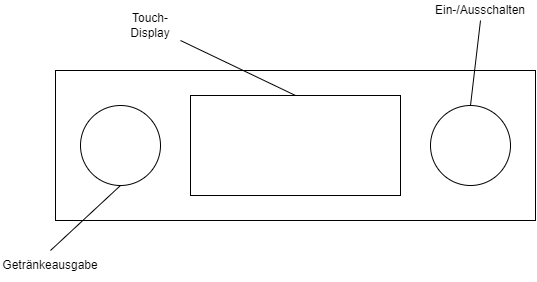
\includegraphics[width=0.8\textwidth]{img/Bilder_Kapitel_2/Bedienungsschnittstelle_Mischmaschine.png}}
    \caption{Schematischer Aufbau der Bedienungsschnittstelle}
    \label{fig:bedienungsschnittstelle_mischmaschine}
\end{figure}
\noindent
Abbildung \ref{fig:bedienungsschnittstelle_mischmaschine} stellt den schematischen Aufbau der Bedienungsschnittstelle der Getränkemischmaschine für ein besseres Verständnis dar.\\\\
Die technische Umsetzung basiert auf der Kommunikation zwischen dem Touch-Display und einem, in der Getränkemischmaschine verbauten, Arduino, der anhand der Daten von der Benutzereingabe, die Pumpen steuert. Beim Drücken des Startknopfes werden das Display und der Arduino mit Strom versorgt, sodass sowohl das Display als auch der Arduino starten und mit der Ausführung des benutzerdefinierten Quelltextes beginnen. Auf dem Bediendisplay findet sich fünf Schieberegler - ein Schieberegler je Behälter - mit denen der Benutzer die Zusammensetzung seines Mischgetränks aus den fünf Behältern konfigurieren kann. Beim Drücken eines in der \ac{UI} des Displays dargestellten Knopfes werden die Werte der Schieberegler an den Arduino übertragen. Dieser rechnet die Prozentwerte der Schieberegler in Durchsatzraten für die Pumpen um. Wird anschließend der Knopf für die Getränkeausgabe gedrückt gehalten steuert der Arduino die Pumpen mit ihrer jeweiligen Durchsatzrate an und der Anwender bekommt sein Mischgetränk ausgegeben.
\section{Hardware}
\section{Sprachverarbeitung}
Im Zuge des technologischen Fortschritts nutzen die Menschen heutzutage zunehmend Sprachassistenten für verschiedene Aufgaben. 
Einer der Hauptvorteile der Sprachsteuerung ist die Bequemlichkeit und Geschwindigkeit, mit der Aufgaben erledigt werden können, ohne dass man tippen oder mit der Maus klicken muss. 
Sprachassistenten nutzen die Verarbeitung natürlicher Sprache, um Befehle zu erkennen und zu verstehen, die der Nutzer laut ausspricht.\\\\
Die Verarbeitung natürlicher Sprache - \ac{NLP} - ist eine wichtige Technologie, die es Computern ermöglicht, die von Menschen verwendete natürliche Sprache zu verstehen. 
Diese Technologie ermöglicht es Computern, menschliche Sprache zu erkennen und zu interpretieren und Text und Sprache in natürlicher Sprache zu erzeugen. 
Im Bereich der Sprachsteuerung spielt \ac{NLP} eine Schlüsselrolle bei der Erkennung von Sprache und dem Verstehen von Befehlen, die der Benutzer laut ausspricht. 
Es wird verwendet, um die Sprache des Benutzers in Text umzuwandeln, den ein Computer verstehen und verarbeiten kann.
Um dies zu erreichen, verwendet \ac{NLP} eine Vielzahl von Techniken und Technologien, darunter maschinelles Lernen, Tonanalyse, syntaktische Analyse und mehr. \cite{jurafsky_speech_2009}\\\\
Im Rahmen dieses Projekts erfordert die Implementierung der Sprachsteuerung einer Getränkemischmaschine die Verarbeitung natürlicher Sprache, damit die Maschine Befehle verstehen kann, die der Benutzer laut ausspricht. 
Dieses Projekt ähnelt einem Chatbot, bei dem der Benutzer eine Frage stellen oder einen Befehl geben kann und der Chatbot führt die entsprechende Aktion aus. 
Die Verarbeitung natürlicher Sprache ist für die Entwicklung eines solchen Sprachsteuerungssystems unerlässlich und ermöglicht es der Maschine, Befehle in natürlicher Sprache zu verstehen und auszuführen.\\\\
Eine der wichtigsten Komponenten der Verarbeitung natürlicher Sprache ist die Spracherkennung und das Syntaxanalyseverfahren. 
Bei der Spracherkennung kommen Deep-Learning-Techniken zum Einsatz, die es einem Computer ermöglichen, Sprachlaute zu erkennen und in Text zu übersetzen. 
Anschließend wird das Syntaxanalyseverfahren verwendet, um die Satzstruktur zu bestimmen und Schlüsselwörter und -sätze hervorzuheben, die zur Bestimmung des Benutzerbefehls verwendet werden können.
Auch die Tonwertanalyse ist ein wichtiger Bestandteil der Verarbeitung natürlicher Sprache. 
Mit Hilfe der Tonalitätsanalyse lässt sich die emotionale Färbung des Textes bestimmen, was für die Ermittlung der Absicht des Nutzers nützlich sein kann. 
Da die Tonwertanalyse im Rahmen dieser Arbeit nicht relevant ist, wird sie nicht weiter erörtert.\\\\
Darüber hinaus werden grammatik- und regelbasierte Technologien zur Verarbeitung natürlicher Sprache eingesetzt. 
Diese Technologien werden eingesetzt, um die korrekte Struktur des Benutzerbefehls zu bestimmen und Schlüsselwörter hervorzuheben, die zur Durchführung von Aktionen verwendet werden können. 
Außerdem werden Techniken des maschinellen Lernens eingesetzt, damit der Computer aus früheren Befehlen und Aktionen \glqq{}lernen\grqq{} kann, was die Genauigkeit der Erkennung von Benutzerbefehlen verbessert.\\\\
Daher ist der Einsatz von Technologien zur Verarbeitung natürlicher Sprache für das Projekt der Sprachmischmaschine unerlässlich. 
Die Verarbeitung natürlicher Sprache wird es der Maschine ermöglichen, die Befehle zu verstehen und zu verarbeiten, die der Benutzer laut ausspricht und die entsprechenden Aktionen durchzuführen.
\subsection{Verarbeitung natürlicher Sprache}
Die Verarbeitung natürlicher Sprache ist ein Forschungsbereich der Informatik und der \ac{KI}, der sich mit der Verarbeitung natürlicher Sprache befasst. 
Bei der Verarbeitung geht es in der Regel darum, natürliche Sprache in Daten zu übersetzen, die ein Computer nutzen kann, um Informationen über die Welt um ihn herum zu erhalten.\\\\
Die \ac{NLP}-Pipeline, die zur Erstellung eines Dialogsystems erforderlich ist, erfordert vier Arten der Verarbeitung sowie eine Datenbank zur Speicherung vergangener Äußerungen und Antworten. 
Jeder dieser Schritte kann einen oder mehrere Verarbeitungsalgorithmen enthalten, die parallel oder sequentiell arbeiten \cite{lane_natural_2019}:
\begin{itemize}
    \item Syntaktische Zergliederung - Extraktion von Merkmalen (strukturierte numerische Daten) aus natürlichem Text.
    \item Analyse - Erstellen und Kombinieren von Items, um Indikatoren für den Ton, die grammatikalische Korrektheit und die Semantik des Textes zu erhalten.
    \item Generierung - Generierung möglicher Antworten mit Hilfe von Mustern, Suchwerkzeugen oder Sprachmodellen.
    \item Ausführung - bereitet Aussagen vor, die auf der Geschichte und dem Zweck des Gesprächs basieren und wählt eine Folgeantwort.
\end{itemize}
\begin{figure}[H]
    \centering
    \fbox{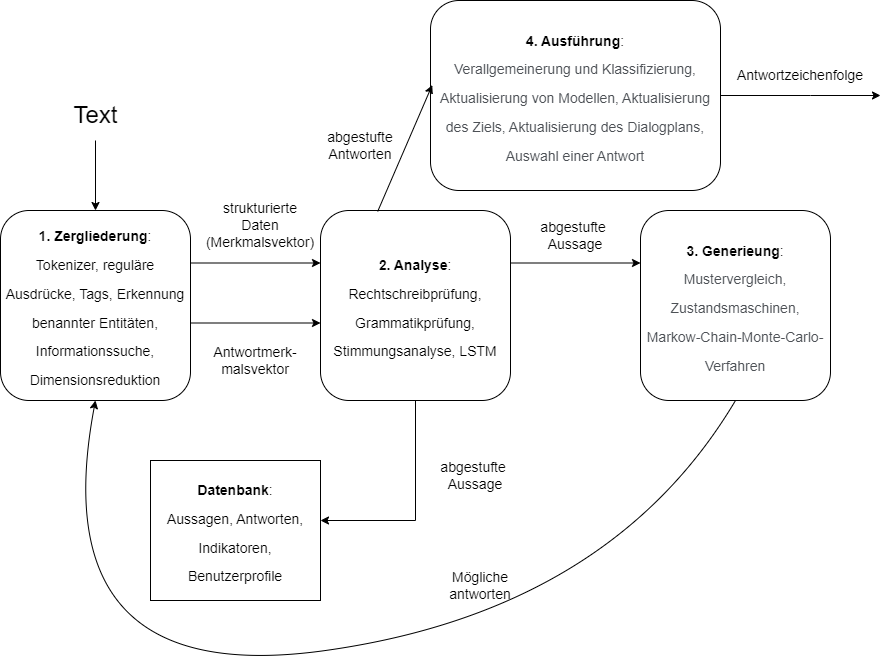
\includegraphics[width=0.8\textwidth]{Bilder_Kapitel_2/Chat-Bot-Pipeline.png}}
    \caption{Rekurrente Chat-Bot-Pipeline}
    \label{figure:Chat-Bot-Pipeline}
\end{figure}
\noindent
Die meisten Chatbots enthalten Elemente aus allen fünf Teilsystemen (die vier Verarbeitungsstufen sowie die Datenbank). 
Viele Anwendungen erfordern jedoch nur einfache Algorithmen, um viele dieser Schritte auszuführen. 
Ein Chatbot oder virtueller Assistent für Verbraucher wie Alexa oder Allo ist in der Regel so konzipiert, dass er äußerst sachkundig und leistungsfähig ist. 
Die Logik, die zur Beantwortung von Anfragen verwendet wird, ist jedoch oft oberflächlich und besteht aus einer Reihe von Codephrasen, die mit einer einzigen if-then-Entscheidungsverzweigung zur gleichen Antwort führen. 
Alexa (und die zugrundeliegende Lex-Engine) verhält sich wie ein einschichtiger, flacher Baum von Operatoren (if, elif, elif...). 
Andererseits stützt sich die Google Translate-Pipeline (oder jedes ähnliche maschinelle Übersetzungssystem) auf eine mehrstufige Hierarchie von Merkmalsextraktoren, Entscheidungsbäumen und Wissensgraphen, die Fragmente von Wissen über die Welt miteinander verbinden.\\\\
Alle \ac{NLP}-Merkmale müssen gut funktionieren, damit das Dialogsystem richtig funktioniert:
\begin{itemize}
    \item Merkmalsextraktion (normalerweise zur Erstellung eines Vektorraummodells).
    \item Informationssuche zur Beantwortung von Sachfragen.
    \item Semantische Suche, um Informationen aus zuvor aufgezeichneten natürlichsprachlichen Texten oder Dialogen zu assimilieren.
    \item Generierung von natürlicher Sprache, um neue sinnvolle Aussagen zu verfassen.
\end{itemize}
\subsection{Tokenisierung von Wörtern}
Eine der wichtigsten Aufgaben der Verarbeitung natürlicher Sprache ist die Tokenisierung, d. h. die Zerlegung von Text in einzelne Wörter oder Phrasen, die so genannten Token. 
Dieser Prozess ist ein wichtiger Bestandteil der Verarbeitung natürlicher Sprache, da er es Programmen und Algorithmen ermöglicht, Texte anhand ihrer Bestandteile zu verstehen und zu analysieren. 
Die Tokenisierung ist für die Verarbeitung natürlicher Sprache von entscheidender Bedeutung, da sie es Programmen ermöglicht, Schlüsselwörter, Phrasen und semantische Einheiten in einem Text hervorzuheben. 
Die Tokenisierung kann auch dazu verwendet werden, nicht benötigte Textelemente wie Satzzeichen, Leerzeichen und andere Zeichen, die keine Bedeutung haben, zu entfernen. 
Dadurch können Programme und Algorithmen effizienter und genauer arbeiten und die Wahrscheinlichkeit von Fehlern und falscher Textverarbeitung verringern.\\\\
Im \ac{NLP} ist die Tokenisierung eine besondere Art der Segmentierung von Dokumenten. 
Bei der Segmentierung wird der Text in kleinere Abschnitte (Segmente) mit engerem Informationsgehalt unterteilt. 
Die Segmentierung kann die Aufteilung eines Dokuments in Absätze, in Sätze, in Phrasen und in Token (Wörter) sowie Satzzeichen umfassen. 
Ein Tokenizer kann mit einem Scanner im Kompilierungsprozess verglichen werden. 
Token sind in diesem Fall die Endpunkte von kontextfreien Grammatiken - \ac{CFG} - zur Analyse von Programmiersprachen-Terminalen.\\\\
Die Tokenisierung ist der erste Schritt in der \ac{NLP}-Pipeline und kann daher den Rest der Pipeline stark beeinflussen. 
Der Tokenizer zerlegt unstrukturierte Daten, d. h. natürlichsprachliche Texte, in Informationseinheiten, die als einzelne Elemente gezählt werden können. 
Die so gezählte Anzahl von Token-Vorkommen in einem Dokument kann direkt als Vektor verwendet werden, der dieses Dokument repräsentiert. 
Ein solcher Ansatz ermöglicht es, aus einer unstrukturierten Zeichenfolge (einem Textdokument) unmittelbar eine für das maschinelle Lernen geeignete numerische Datenstruktur zu gewinnen. 
Diese Werte können den Computer direkt dazu veranlassen, nützliche Aktionen durchzuführen und Reaktionen zu erzeugen.\\\\
Die einfachste Art, einen Satz zu tokenisieren, ist die Verwendung von Leerzeichen als Worttrenner in Zeichenketten. 
Dies ist jedoch nicht optimal, denn wenn ein Satz z. B. ein Satzzeichen enthält, wird es von einem der Tokenisierer erfasst. 
Optimierte Tokenizer sind in mehreren Python-Bibliotheken implementiert, die jeweils ihre eigenen Vor- und Nachteile haben: spaCy, Stanford CoreNLP und \ac{NLTK}. 
\ac{NLTK} und StanfordCoreNLP sind die am längsten bestehenden und am häufigsten verwendeten Bibliotheken zum Vergleich von \ac{NLP}-Algorithmen in wissenschaftlichen Artikeln. 
Obwohl die StanfordCoreNLP-Bibliothek eine Python-\ac{API} hat, basiert sie auf dem Java 8 CoreNLP-Anwendungsteil, der separat installiert und konfiguriert werden muss. 
Daher wurde in dieser Arbeit der \ac{NLTK}-Tokenizer verwendet.\\\\
Ein wichtiges Konzept im Tokenisierungsprozess sind N-Gramme. 
Ein N-Gramm ist eine Sequenz mit bis zu n Elementen, die aus einer Sequenz dieser Elemente, in der Regel einer Zeichenkette, extrahiert wurden. 
Im Allgemeinen können die Elemente eines N-Gramms Buchstaben, Silben, Wörter oder sogar Symbole sein. 
N-Gramme sind notwendig, weil bei der Konvertierung einer Menge von Wörtern in einen Vektor eine Folge von Token einen Großteil der Bedeutung verliert, die in der Reihenfolge dieser Wörter verkapselt ist. 
Wenn das Token-Konzept auf Mehrwort-Token, N-Gramme, ausgedehnt wird, kann die \ac{NLP}-Pipeline einen erheblichen Teil der Bedeutung, die in der Wortfolge dieser Äußerungen enthalten ist, beibehalten. 
So bleibt beispielsweise das Wort \glqq{}kein\grqq{}, das die Bedeutung umkehrt, neben den benachbarten Wörtern stehen, wo es hingehört. 
Ohne N-Gramm-Tokenisierung würde ein solches Wort an verschiedenen Positionen herumhängen und seine Bedeutung würde mit dem gesamten Satz oder Dokument assoziiert werden, anstatt mit benachbarten Wörtern. 
Das Bigramm \glqq{}war nicht\grqq{} behält viel mehr Bedeutung der einzelnen Wörter \glqq{}war\grqq{} und \glqq{}nicht\grqq{} als die entsprechenden Singlegramme im Multigrammvektor. 
Durch die Verknüpfung eines Wortes mit seinen Nachbarn in einem Förderband kann ein Teil seines Kontexts erhalten bleiben. 
N-Gramme sind also ein Instrument zur Speicherung von Kontextinformationen, während die Daten die Pipeline durchlaufen.\\\\
Die Größe des Vokabulars spielt eine wichtige Rolle für die Leistung der \ac{NLP}-Pipeline. 
Die Größe des Wörterbuchs bestimmt die Größe der Trainingsstichprobe, die benötigt wird, um eine Überanpassung an ein bestimmtes Wort oder eine bestimmte Phrase zu vermeiden und die Größe der Trainingsmenge bestimmt die Kosten der Verarbeitung. 
Eine Technik zur Verringerung der Größe des Wörterbuchs besteht darin, Token, die ähnliche Dinge bedeuten, in einer einzigen normalisierten Form zusammenzufassen. 
Eine solche Technik reduziert die Anzahl der gespeicherten Token und verbessert die Verbindungen zwischen den Bedeutungen von Phrasen mit unterschiedlicher \glqq{}Schreibweise\grqq{} der Tokens und verringert die Wahrscheinlichkeit des Überlernens. 
Eine der Normalisierungsmöglichkeiten ist die Groß- und Kleinschreibung - die Kombination mehrerer Schreibweisen eines Wortes, die sich nur in der Groß- und Kleinschreibung unterscheiden. 
In diesem Fall wird die Groß-/Kleinschreibung ignoriert und zwei identische Wörter, von denen eines groß und das andere klein geschrieben wird, werden als dasselbe Token behandelt.\\\\
Ein weiterer wichtiger Schritt bei der Tokenisierung von Texten ist die Entfernung von Stoppwörtern, um den Umfang des Wörterbuchs zu verringern. 
Stoppwörter sind in jeder Sprache gebräuchliche Wörter, die sehr häufig vorkommen, aber sehr viel weniger aussagekräftige Informationen über die Bedeutung eines Satzes enthalten (z. B. a, an, the, this, of, on im Englischen oder der, die, das, diese im Deutschen). 
Stoppwörter können jedoch nützliche Informationen enthalten, so dass man sie nicht immer verwerfen sollte. 
Das \ac{NLTK}-Paket für Python enthält derzeit die umfassendste Liste kanonischer Stoppwörter in verschiedenen Sprachen.\\\\
Eine weitere gängige Methode der Normalisierung ist die Beseitigung kleiner semantischer Unterschiede im Zusammenhang mit Pluralendungen und Possessivendungen von Wörtern oder sogar unterschiedlichen Verbformen. 
Diese Methode der Normalisierung, bei der ein gemeinsamer Wortstamm für verschiedene Wortformen gefunden wird, wird als Stemming bezeichnet. 
Der gemeinsame Wortstamm von \glqq{}Gehäuse\grqq{} und \glqq{}Haus\grqq{} ist zum Beispiel \glqq{}Haus\grqq{}.
 Beim Stemming werden Suffixe von Wörtern entfernt, um Wörter mit ähnlicher Bedeutung unter einem gemeinsamen Stamm zu gruppieren. 
 Der Wortstamm muss nicht unbedingt ein gültiges Wort sein, sondern kann auch nur ein Token oder eine Bezeichnung sein, das mehrere mögliche Schreibweisen repräsentiert. 
 Einer der Hauptvorteile des Stemming besteht darin, die Anzahl der Wörter zu verringern, deren Bedeutung das Sprachmodell im Auge behalten muss. 
 Durch diese Methode wird die Größe des Wörterbuchs reduziert, wodurch der Verlust nützlicher Informationen und Bedeutungen so weit wie möglich begrenzt wird. 
 Das Stemming spielt eine wichtige Rolle bei der Suche nach Schlüsselwörtern oder Informationen. 
Zwei der bekanntesten Algorithmen sind Porter's Stemmer und Snowball.\\\\
Mit Informationen über die Beziehungen zwischen den Bedeutungen verschiedener Wörter ist es möglich, mehrere Wörter miteinander zu verknüpfen, auch wenn ihre Schreibweise sehr unterschiedlich ist. 
Eine solche erweiterte Normalisierung eines Wortes auf seine semantische Wurzel - ein Lemma - wird Lemmatisierung genannt. 
Die Lemmatisierung ist potenziell eine viel genauere Art der Normalisierung als das Stemming oder die Groß- und Kleinschreibung, da sie die Bedeutung des Wortes berücksichtigt. 
Der Lemmatisierer verwendet eine Wissensbasis von Synonymen und Wortendungen, um nur eng verwandte Wörter zu einem Token zu kombinieren. 
In Python kann die Lemmatisierung mit dem \ac{NLTK}-Paket implementiert werden, das den \textit{WordNetLemmatizer} enthält.\\\\
Wie bereits gezeigt wurde, ist die Tokenisierung der Prozess der Zerlegung von Text in einzelne Wörter oder Token. 
Für viele Anwendungen der Verarbeitung natürlicher Sprache ist jedoch nicht nur wichtig, welche Wörter im Text enthalten sind, sondern man muss auch in der Lage sein, diese Wörter als Zahlen darzustellen. 
Dadurch wird es möglich, maschinelles Lernen und andere Algorithmen, die mit Zahlen arbeiten, zur Textverarbeitung einzusetzen. 
Bei der Verarbeitung natürlicher Sprache wird dazu die Wortvektorisierung verwendet.
\subsection{Vektorisierung von Wörtern}
Die Vektorisierung hilft dabei, eine numerische Darstellung zu finden, die die Bedeutung oder den Informationsgehalt der dargestellten Wörter widerspiegelt. 
Es gibt drei Möglichkeiten, Wörter und ihre Bedeutungen darzustellen:
\begin{itemize}
    \item Multisets von Wörtern - Vektoren von Zahlen oder Häufigkeiten von Wörtern. 
    \item Multisets von N-Grammen - Vektoren von Mengen von Wortpaaren (Bigramme), Worttripeln (Trigramme), usw.
    \item TF-IDF-Vektoren sind Indikatoren für Wörter, die deren Bedeutung am Besten darstellen.
\end{itemize}
Jede dieser Methoden kann entweder allein oder als Teil einer \ac{NLP}-Pipeline angewendet werden. 
Alle beschriebenen Modelle sind statistisch in dem Sinne, dass sie auf Worthäufigkeiten beruhen.\\\\
\ac{BOW}-Vektoren sind Vektoren, die Textdokumente als Wort-Multisets (Bags) darstellen, wobei ein Multiset eine Sammlung von Elementen ist, in der jedes Element mehr als einmal wiederholt werden kann. 
Ein Wort-Bag ist eine Darstellung von Text, die das Vorkommen von Wörtern in einem Dokument beschreibt. 
Sie beinhaltet zwei Dinge:
\begin{enumerate}
    \item Ein Wörterbuch mit bekannten Wörtern.
    \item Ein Maß für das Vorhandensein von bekannten Wörtern.
\end{enumerate}
Dies wird als "Wort-Bag" bezeichnet, weil alle Informationen über die Reihenfolge oder Struktur der Wörter im Dokument verworfen werden. 
Das Modell interessiert sich nur dafür, ob bekannte Wörter im Dokument vorkommen, nicht aber, wo im Dokument. 
Bei diesem Ansatz wird das Histogramm der Wörter im Text betrachtet, d. h. wir betrachten jedes Wort als ein Merkmal \cite{goldberg_neural_2017}.\\\\
Ein Ansatz zur Vektorisierung einer Vielzahl von Wörtern besteht darin, für jedes Wort einen Einheitsvektor zu erstellen und diese Vektoren dann zu einem einzigen Vektor zu kombinieren. 
Ein unitärer Vektor für ein Wort ist ein Vektor, dessen Länge der Dimension des Raumes entspricht und alle seine Komponenten sind Null, mit Ausnahme einer Komponente, die der Position des Wortes im Wörterbuch entspricht. Unitäre Vektoren sind extrem spärlich. 
Enthält das Wörterbuch beispielsweise 1000 Wörter, dann hat jeder unitäre Vektor eine Dimension von 1000 und die Komponente, die der Position des Wortes im Wörterbuch entspricht, ist gleich eins.
Zum Beispiel sieht der unitäre Vektor für den Satz \glqq Mojito ist ein leckerer Cocktail\grqq{} (nach dem Tokenisierungsprozess) so aus:
\begin{figure}[H]
    \centering
    \fbox{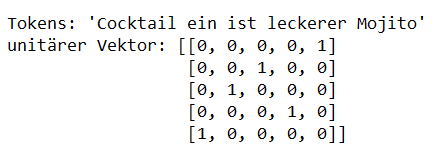
\includegraphics[width=0.6\textwidth]{Bilder_Kapitel_2/unitaerer_vektor.png}}
    \caption{\label{figure:Unitaere_Vektoe}Unitärer Vektor}
\end{figure}
\noindent
Eine der Eigenschaften der vektoriellen Darstellung von Wörtern und der tabellarischen Darstellung von Dokumenten ist, dass keine ursprünglichen Informationen verloren gehen. 
Das Originaldokument kann aus dieser einheitlichen Vektortabelle rekonstruiert werden. 
Daher werden solche unitären Vektoren in neuronalen Netzen, bei der \ac{seq2seq}-Modellierung und bei der Erstellung von Sprachmodellen verwendet. 
Unitäre Vektoren eignen sich hervorragend für alle \ac{NLP}-Modelle oder -Pipelines, bei denen die Bedeutung des Ausgangstextes vollständig erhalten bleiben muss.
\subsection{Syntaktische Analyse}
\subsection{Ansätze für die Erstellung eines Chatbots}\label{sec:ansaetze_erstellung_chatbots}
Derzeit gibt es vier Hauptansätze für die Erstellung eines Chatbots \cite{lane_natural_2019}:
\begin{itemize}
    \item Musterabgleich: Musterabgleich und Antwortvorlagen (vorgefertigte Antworten)
    \item Grounding: logische Wissensgraphen und das Ziehen von Schlussfolgerungen aus diesen basierend auf diesen Graphen
    \item Suche: Abrufen von Text
    \item Generierungsmethoden: Statistik und maschinelles Lernen
\end{itemize}
Die vier grundlegenden Ansätze zur Erstellung von Chatbots lassen sich kombinieren, was zu benutzerfreundlicheren Chatbots führt. 
Eine Vielzahl von Anwendungen nutzen alle vier grundlegenden Methoden. 
Hybride Chatbots unterscheiden sich hauptsächlich darin, wie genau sie diese Ansätze kombinieren und wie viel Gewicht auf jeden einzelnen Ansatz gelegt wird.
\subsubsection{Musterabgleich}
Bei den ersten Chatbots basierte die Antwort auf die Nachricht eines Benutzers auf einem Mustervergleich. 
Diese Chatbots suchen nach Mustern im eingehenden Text und geben eine feste (gemusterte) Antwort, wenn eine Übereinstimmung gefunden wird \cite{woudenberg_chatbot_2014}.\\\\
Solche rudimentären Dialogsysteme sind vor allem in automatisierten Benutzerunterstützungssystemen mit interaktiven Sprachmenüs nützlich, wo es möglich ist, das Gespräch an einen Menschen weiterzuleiten, wenn der Chatbot keine Antwortmuster mehr hat.\\\\
Da es viele \ac{NLP}-Dienstprogramme in Python-Paketen gibt, ist es möglich, komplexere Chatbots auf der Grundlage von Mustervergleichen zu erstellen, indem man die Bot-Logik nach und nach direkt in Python mit regulären Ausdrücken und Suchmustern aufbaut.\\\\
1995 machte sich Richard Wallace daran, einen allgemeinen Rahmen für die Erstellung von Chatbots auf der Grundlage des Pattern-Matching-Ansatzes zu schaffen. Zwischen 1995 und 2002 schuf seine Entwicklergemeinschaft die \ac{AIML} zur Beschreibung von Mustern und Chatbot-Antworten.\\\\
\ac{AIML} ist eine deklarative Sprache, die auf dem \ac{XML}-Standard basiert, der die Sprachkonstrukte und Datenstrukturen einschränkt, die im Bot verwendet werden dürfen. \cite{noauthor_aiml_nodate}
Ein Chatbot, der auf \ac{AIML} basiert, sieht folgendermaßen aus:
\begin{figure}[H]
    \centering
    \fbox{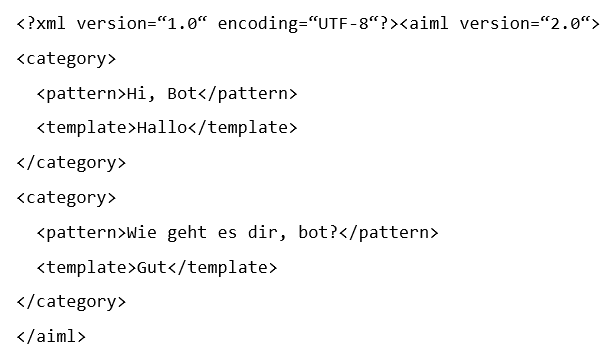
\includegraphics[width=0.8\textwidth]{Bilder_Kapitel_2/aiml_bot.png}}
    \caption{\label{figure:Aiml_Bot}\ac{AIML} Chatbot}
\end{figure}
\noindent
Eine der Einschränkungen von \ac{AIML} ist die Art der Muster, die abgeglichen werden können und auf die reagiert wird. 
Der \ac{AIML}-Kern (Pattern Matching Engine) reagiert nur auf Eingabetext, der einem vom Entwickler manuell vorgegebenen Muster entspricht. 
Unscharfe Suchanfragen, Smileys, Satzzeichen, Tippfehler oder falsch geschriebene Wörter sind nicht erlaubt, es findet kein automatischer Abgleich statt. 
In \ac{AIML} müssen alle Synonyme manuell einzeln beschrieben werden.
\subsubsection{Grounding}
Die Grounding-Methode ist ein Ansatz zur Erstellung eines Chatbots auf der Grundlage logischer Wissensgraphen und der Durchführung von Schlussfolgerungen auf der Grundlage dieser Graphen. \cite{diana_conversational_2011}
Sie wird verwendet, um natürliche Sprache zu verarbeiten und sie dem Verständnis des Bots zuzuordnen. Das Wesentliche an der Grounding-Methode ist, dass der Chatbot nicht nur die Textnachrichten, sondern auch den Kontext und die Umgebung verarbeitet, um Anfragen besser zu verstehen und zu beantworten. 
Durch die Extraktion von Informationen wird ein Netz von Verbindungen oder Fakten geschaffen. Dieses Netz logischer Verbindungen zwischen Entitäten - ein Graph oder eine Wissensbasis - kann die Grundlage für die Antworten des Chatbots bilden.\\\\
Ein Beispiel für eine Grounding-Methode ist die Verwendung eines Wissensgraphen zur Beschreibung der Umgebung. 
Ein Wissensgraph enthält Informationen über die Objekte, mit denen der Bot interagieren kann und die Beziehungen zwischen ihnen. 
Ein Wissensgraph könnte zum Beispiel Informationen über ein Glas auf einem Tisch und das darin befindliche Wasser enthalten. 
Wenn ein Benutzer eine Frage stellt, verwendet der Chatbot den Wissensgraphen, um den Kontext der Anfrage zu verstehen und die am besten geeignete Antwort abzuleiten. 
Wenn ein Benutzer zum Beispiel fragt: \glqq{}Wie hoch ist die Temperatur des Wassers in dem Glas auf dem Tisch?\grqq{}, kann der Chatbot Informationen aus dem Wissensgraphen verwenden, um die Frage zu beantworten.\\\\
Ein solcher Wissensgraph kann abgeleitet werden, um Fragen über die in dieser Wissensbasis enthaltene Welt zu beantworten und anschließend können auf der Grundlage der logischen Antworten die Werte der in den Antworten enthaltenen Template-Variablen ausgefüllt werden, um natürlichsprachliche Antworten zu erstellen. 
Ursprünglich wurden auf diese Weise Systeme zur Beantwortung von Fragen eingerichtet, wie z. B. der Watson-Bot von IBM (heutzutage wird für ähnliche Systeme jedoch die Informationssuchemethode verwendet). 
Der Wissensgraph stellt eine Art \glqq{}Erdung\grqq{} des Chatbots in der realen Welt dar.\\\\
Die Erstellung von Chatbots auf der Grundlage von \glqq{}Grounding\grqq{} eignet sich hervorragend für Chatbots, die Fragen generieren, bei denen das zur Beantwortung einer Frage erforderliche Wissen in einer umfangreichen Wissensbasis enthalten ist, die aus einer offenen Datenbank (z. B. Wikidata, Open Mind Common Sense oder DBpedia) bezogen werden kann.\\\\
Einer der Hauptvorteile der Grounding-Methode besteht darin, dass sie sich an ein sich veränderndes Umfeld anpassen kann. 
Wenn der Benutzer zum Beispiel ein Glas Wasser von einem Tisch auf einen anderen stellt, wird der Wissensgraph automatisch aktualisiert, um diese Änderung widerzuspiegeln.\\\\
Die Grounding-Methode hat jedoch auch ihre Grenzen. 
So kann es vorkommen, dass bei der Verarbeitung großer Informationsmengen Zusammenhänge nicht berücksichtigt werden und dem Bot möglicherweise verborgen bleiben.\\\\
Insgesamt ist die Grounding-Methode ein effektiver Ansatz zur Erstellung wissensbasierter Chatbots. 
Sie ermöglicht es dem Bot, Benutzeranfragen besser zu verstehen und eine genauere Antwort zu geben.
\subsubsection{Suche}
Die Informationssuchemethode ist eine der Methoden zum Aufbau von Chatbots, die auf der Extraktion von Informationen aus einer großen Menge von Textinformationen basiert. 
Die Hauptidee der Informationssuchemethode ist die Analyse des Eingabetextes (Benutzeranfrage), die Auswahl von Schlüsselwörtern und Phrasen daraus und die anschließende Suche nach den relevantesten Informationen in der Wissensdatenbank oder in offenen Quellen. \cite{diana_conversational_2011}\\\\
Die Wissensbasis kann auch eine Art \glqq{}Gesprächsprotokoll\grqq{} sein, in Form von Aussage-Antwort-Paaren. 
Dabei sucht der Bot nach früheren Aussagen in den Protokollen früherer Unterhaltungen. 
Der Bot kann nicht nur in den Protokollen seiner eigenen Gespräche suchen, sondern auch in beliebigen Transkripten von Gesprächen zwischen Menschen, Gesprächen zwischen Menschen und Bots oder sogar Gesprächen zwischen Bots.
Aber wie immer gilt: je besser die Eingabedaten, desto besser das Ergebnis. 
Daher ist es notwendig, die Datenbank früherer Gespräche sorgfältig zu säubern und zu organisieren, damit der Bot nach einem qualitativ hochwertigen Gespräch sucht und es dann imitiert.\\\\
Für die Umsetzung der Informationssuchemethode werden verschiedene Algorithmen und Techniken verwendet, z. B. Indizierung und Schlagwortsuche, Kontextsuche, Textanalyse mit Hilfe von maschinellen Lernverfahren usw. 
Die Informationssuchemethode kann in Python mit verschiedenen Bibliotheken und Tools wie \ac{NLTK}, Scikit-learn und Gensim implementiert werden.\\\\
Einer der ersten Schritte bei der Implementierung einer Informationssuchemethode in Python ist die Vorbereitung der Daten. 
Dies erfordert Tokenisierung, Lemmatisierung und die Entfernung von Stopp-Wörtern. 
Als nächstes muss ein Index auf der Grundlage von Schlüsselwörtern erstellt werden. 
Der Index kann auf der Grundlage von Bag-of-Words oder \ac{TF} und \ac{IDF} (TF-IDF-Modelle) erstellt werden. 
Sobald der Index erstellt ist, kann eine Stichwortsuche durchgeführt werden. 
Dazu muss die Benutzeranfrage in einen Vektor umgewandelt und mit den Dokumentvektoren im Index verglichen werden. 
Dies kann mit Hilfe der Scikit-learn-Bibliothek erfolgen \cite{scikit-learn}.
Sobald die relevantesten Dokumente gefunden wurden, können sie in eine Rangfolge gebracht und als Antwort auf die Benutzeranfrage angezeigt werden.\\\\
Der Vorteil der Informationssuchemethode besteht darin, dass sie ein schnelles und genaues Auffinden der gewünschten Informationen ermöglicht, insbesondere wenn die Wissensbasis gut strukturiert ist und genügend Informationen enthält. 
Ein Nachteil dieser Methode ist jedoch, dass sie den Kontext der Anfrage nicht berücksichtigt und nicht immer eine vollständige und genaue Antwort auf die Frage des Nutzers liefert. 
Wenn die Aussage semantisch mit der vom Bot zu beantwortenden übereinstimmt, ist es möglich, die Antwort wortwörtlich und ohne Änderungen wiederzuverwenden. 
Aber selbst wenn die Datenbank alle möglichen Benutzeräußerungen enthält, wird der Bot die Persönlichkeiten der Personen widerspiegeln, die diese Äußerungen machen. 
Wenn die Antworten konsistent sind und von einer Vielzahl von Personen stammen, ist das gut. 
Problematisch wird es jedoch, wenn die Äußerung, auf die der Bot reagieren soll, vom Gesamtkontext des jeweiligen Gesprächs oder von den Umständen in der Umgebung abhängt, die sich seit der Erstellung des Dialogkorpus geändert haben können.\\\\
Beispielsweise sollte der Bot auf die Frage \glqq{}Wie spät ist es?\grqq{} nicht die von der Person gegebene Antwort, sondern die am besten geeignete Aussage aus der Datenbank verwenden. 
Diese Antwort funktioniert nur, wenn die Zeit, zu der die Frage gestellt wurde, mit der Zeit übereinstimmt, zu der die passende Äußerung aus der Datenbank aufgezeichnet wurde. 
Neben dem natürlichsprachlichen Text der Äußerung müssen auch ähnliche Informationen über die Zeit - der Kontext (Zustand) - erfasst und verglichen werden. 
Sie spielt vor allem dann eine wichtige Rolle, wenn die Semantik der Äußerung auf eine aktive Veränderung des im Kontext (Wissensbasis des Chatbots) erfassten Zustands hinweist.\\\\
Um den Zustand (Kontext) in einem Chatbot auf der Grundlage der Informationssuche zu berücksichtigen, kann etwas Ähnliches für einen Chatbot mit Musterabgleich durchgeführt werden, da die Auflistung einer Liste von Benutzeraussagen nur eine andere Art ist, ein Muster zu beschreiben. 
Dies auch ist der Ansatz von Amazon Lex \cite{amazon_lex} und Google Dialogflow \cite{dialogflow_chawla}. 
Anstatt ein starres Muster zu beschreiben, um den Befehl des Benutzers zu erfassen, können der Dialogflow-Engine einfach ein paar Beispiele geliefert werden. 
So wie jedes Muster im Chatbot auf der Grundlage der Musterzuordnung einem Zustand zugeordnet wurde, muss auch hier nur die Aussage-Antwort-Beispielpaare mit dem genannten Zustand verknüpft werden.\\\\
Der suchbasierte Chatbot indiziert also den Korpus der Dialoge, so dass er leicht frühere Aussagen finden kann, die derjenigen ähnlich sind, auf die er antworten muss und antwortet dann mit einer der passenden Aussagen aus dem Korpus, die er sich \glqq{}gemerkt\grqq{} und für eine schnelle Suche indiziert hat. 
Im Allgemeinen ist die Methode der Informationssuche eine der gängigsten und beliebtesten Methoden zum Aufbau von Chatbots, die in verschiedenen Bereichen wie Wirtschaft, Medizin, Tourismus und vielen anderen eingesetzt werden.
\subsubsection{Generierungsmethoden}
Generierungsmethoden sind einer der wichtigsten Ansätze bei der Entwicklung von Chatbots auf der Grundlage künstlicher Intelligenz. 
Sie ermöglichen es Chatbots, Textantworten auf der Grundlage der Analyse der eingehenden Nachricht und des Kontextes des Dialogs zu generieren. 
Die folgenden Generierungsmodelle sind nützlich, um einen kreativen Chatbot zu erstellen, der Dinge sagen kann, die noch niemand zuvor gesagt hat:
\begin{itemize}
    \item Sequenz-zu-Sequenz-Konvertierungsmodelle: Modelle, die darauf trainiert sind, Antworten auf der Grundlage von Eingabesequenzen zu generieren;
    \item \ac{RBM}: Markov-Ketten, die so trainiert werden, dass sie die \glqq{}Energie\grqq{}-Funktion minimieren \cite{chatbot_development_sharma};
    \item \ac{GAN}: statistische Modelle, die darauf trainiert sind, einen Experten, der die Qualität eines Gesprächs bewertet, zu täuschen. \cite{li_adversarial_2017}
\end{itemize}
Die Vorteile des Einsatzes der Generierungsmethoden:
\begin{itemize}
    \item Flexibilität: Generative Methoden können für eine breite Palette von Aufgaben eingesetzt werden, einschließlich Texterstellung, Sprachübersetzung, Verarbeitung natürlicher Sprache und mehr.
    \item Automatisierung: Generative Methoden können auf großen Datensätzen trainiert werden, wodurch die Erstellung von Inhalten automatisiert werden kann.
    \item Qualität: Generative Methoden zeigen eine hohe Qualität bei der Textgenerierung, Sprachübersetzung und anderen Aufgaben der natürlichen Sprachverarbeitung, wenn sie auf einem ausreichend großen Datensatz trainiert werden.
    \item Schnelligkeit: Generative Methoden können schneller arbeiten als Menschen, was die Erstellung von Inhalten mit großer Geschwindigkeit ermöglicht.
\end{itemize}
Die Nachteile der generativen Methoden:
\begin{itemize}
    \item Große Datenmengen für das Training: Generative Methoden benötigen große Datenmengen für das Training, was bei einigen Aufgaben schwierig sein kann, insbesondere wenn nur ein kleiner Datensatz zur Verfügung steht.
    \item Sicherheitsrisiken: Generative Methoden können Inhalte erzeugen, die möglicherweise falsch, unvollständig oder irreführend sind. Dies kann zu Sicherheitsrisiken führen, wenn der generierte Inhalt für wichtige Entscheidungen verwendet wird.
    \item Unterstützungsbedarf: Generative Methoden können erhebliche Unterstützung benötigen, um effektiv zu sein. Dies kann die Modellabstimmung, die Auswahl optimaler Parameter und die Optimierung der Modellleistung auf einer bestimmten Hardwarekonfiguration umfassen.
    \item Modellbeschränkungen: Generative Methoden können Beschränkungen hinsichtlich der Arten von Inhalten haben, die sie erzeugen können, insbesondere wenn sie nur auf bestimmte Datentypen trainiert wurden.
\end{itemize}
Eine der beliebtesten Methoden zur Texterstellung ist die sequence-to-sequence-Methode (seq2seq). 
Die seq2seq-Methode basiert auf \ac{RNN}, die die Simulation von Datenfolgen ermöglichen. 
Sie besteht aus zwei Hauptteilen: einem Encoder und einem Decoder. 
Ein Encoder empfängt eine Wortfolge und baut daraus einen Kontextvektor auf, der Informationen über die Eingabedaten enthält. 
Der Decoder erhält diesen Vektor als Eingabe und beginnt mit der Generierung einer Folge von Antwortnachrichten, wobei er schrittweise den Kontext und die zuvor generierten Wörter berücksichtigt. \cite{seq2seq_alammar}\\\\
Einer der Hauptvorteile der seq2seq-Methode ist ihre Fähigkeit, qualitative und grammatikalisch korrekte Textantworten zu generieren, einschließlich Antworten, die nicht in den Trainingsdaten enthalten waren. 
Sie kann auch mit langen Sequenzen umgehen, was sie ideal für die Generierung von Antworten in Dialogsystemen macht. 
Darüber hinaus kann die seq2seq-Methode in einer Vielzahl von Anwendungen eingesetzt werden, z. B. in der maschinellen Übersetzung, der Spracherkennung und anderen.\\\\
Die seq2seq-Methode hat jedoch ihre Nachteile. 
Sie erfordert große Datenmengen zum Trainieren und Verarbeiten sowie erhebliche Rechenressourcen. 
Dies kann die Anwendung der Methode bei einigen Anwendungen einschränken. 
Wenn der Trainingsdatensatz nicht eine ausreichend große Bandbreite möglicher Antworten repräsentiert, kann das Modell außerdem dazu neigen, vorhersehbare oder falsche Antworten zu erzeugen.\\\\
Die Implementierung der seq2seq-Methode in Python kann mit der TensorFlow-Bibliothek erfolgen, die eine Reihe von Werkzeugen für den Aufbau und das Training neuronaler Netze bietet. 
In TensorFlow kann man die vortrainierten seq2seq-Modelle verwenden oder ein eigenes Modell erstellen, indem die Architektur und die Trainingsparameter des Netzwerks konfiguriert wird. \cite{tensorflow}
\endinput
\chapter{Konzept} \label{chap:konzept}
In diesem Kapitel wird zunächst erläutert, wie die Steuerung der Getränkemischmaschine durch Sprachbefehle im Allgemeinen ablaufen wird.
Anschließend werden mehrere Konzepte vorgestellt, die das allgemeine Konzept konkretisieren.
Diese werden anhand der, in Kapitel \ref{section:Bewertungskriterien} erläuterten Kriterien, bewertet.
Zuletzt wird die Wahl des finalen Konzepts begründet.
\section{Allgemein}
Der Benutzer soll über Spracheingaben mit der Mischmaschine interagieren können.
Dafür muss das Gesprochene zunächst durch ein Mikrofon aufgenommen werden.
Anschließend können die Audiosignale weiterverarbeitet werden.
Der Benutzer soll hierbei nicht auf fest vorgegebene Sprachbefehle beschränkt sein, sondern für nahezu jede Eingabe eine sinnvolle Antwort zurückerhalten.
Um dies zu gewährleisten wird die Spracheingabe durch ein Sprachmodell, welches mittels maschinellen Lernverfahren trainiert wurde, verarbeitet.
Ergebnisse dieser Verarbeitung sind die Antwort, die an den Benutzer zurückgegeben wird, und ein konkreter Befehl für die Mischmaschine.
Ein Beispiel für einen solchen Befehl könnte etwa die Zubereitung eines bestimmten Getränks sein.
Für die Ausgabe einer Antwort ist ein Lautsprecher notwendig.
Denkbar wäre auch eine textbasierte Ausgabe, allerdings ginge damit der Eindruck des Benutzers verloren eine echte Konversation mit der Mischmaschine zu führen.
Das Sprachmodell mit der Getränkemischmaschine zu verknüpfen stellt eine Herausforderung dieser Arbeit dar.
\section{Bewertungskriterien} \label{section:Bewertungskriterien}
Im Folgenden sind die Bewertungskriterien für die einzelnen Konzepte aufgelistet:
\begin{itemize}
    \item Freiheitsgrade in der Spracheingabe des Benutzers: Erhält der Benutzer passende Antworten zurück egal was er sagt oder ist er auf einige wenige Befehle beschränkt?
    \item Hardwarekosten: Wie kostspielig ist das Konzept bezüglich der zusätzlich benötigten Hardware?
    \item Verfügbare Rechenleistung: Wie hoch ist die Verfügbare Rechenleistung im Vergleich zu den anderen Konzepten? Reicht diese aus um das Sprachmodell auszuführen?
    \item Performanz: Als wie performant wird die Lösung eingeschätzt? Ist mit Latenzen zwischen der Einagbe des Benutzers, der Ausgabe einer Antwort und Ausführung der Aktion zu rechnen?
    \item Overhead: Wie hoch ist im Allgemeinen der Mehraufwand einzuschätzen?
\end{itemize}
\section{Konzept A: Spracherkennung und -verarbeitung mittels Arduino} \label{section:Konzept_A}
Ein erstes Konzept sieht vor, dass das Audiosignal direkt von einem der Arduinos in der Getränkemischmaschine aufgenommen wird.
Das Audiosignal wird vom Arduino interpretiert und eine passende Antwort wird ausgegeben.
Außerdem sendet der Arduino die entsprechenden Signale, um die vom Benutzer gewünschte Aktion von der Getränkemischmaschine ausführen zu lassen.
Ein Problem ist hierbei die Interpretation des Audiosignals durch den Arduino, da dessen Leistung nicht für das Ausführen eines Sprachmodells ausreicht.
Folglich muss dieser Prozess ausgelagert werden.
Das Konzept wird deshalb um ein cloudbasiertes Sprachverarbeitungssystem ergänzt, welches den Sprachbefehl des Benutzers vom Arduino entgegennimmt und einen passenden Befehl und eine passende Antwort zurückgibt (s. Abb. \ref{figure:Spracherkennung_mittels_Arduino}).
Die Kommunikation zwischen Arduino und Cloudsystem kann über das \ac{HTTP} erfolgen.
\begin{figure}[H]
    \centering
    % \includegraphics does not allow jpg images apparently!
    \fbox{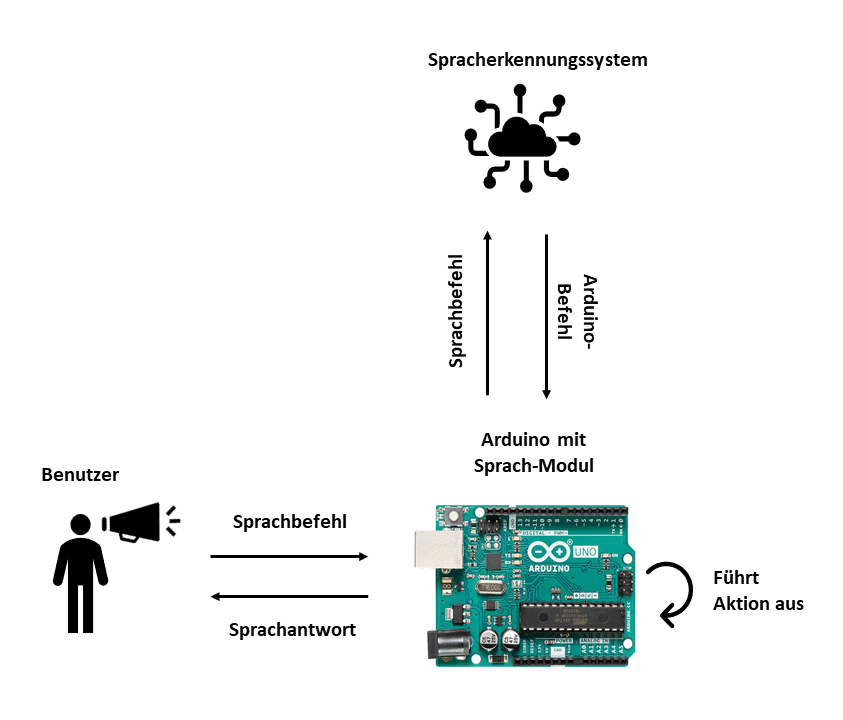
\includegraphics[width=0.8\textwidth]{Bilder_Konzept/Konzept_A.png}}
    \caption{\label{figure:Spracherkennung_mittels_Arduino}Spracherkennung und -verarbeitung mittels Arduino}
\end{figure}
\noindent
Es muss ein geeignetes Format zum Versenden des Sprachbefehls über \ac{HTTP} gefunden werden.
Eine Möglichkeit besteht darin, das eingehende Audiosignal im Arduino in textform umzuwandeln und diesen String zu versenden.
Die auf dem Markt verfügbaren Arduino-Sprach-Module sind jedoch nicht in der Lage beliebige Spracheingaben in Text umzuwandeln, sondern bieten diese Funktionalität nur für vordefinierte Werte an.
Dies würde das Ziel dieser Arbeit verfehlen, dem Benutzer eine Konversation mit der Mischmaschine zu ermöglichen.
Ein weiteres Problem dieser Lösung besteht darin, dass beispielsweise bei wechselnder Getränkeauswahl die zur Verfügung stehenden Sprachbefehle wie "`Ich hätte gerne Getränk xy"' jedes Mal aufs neue manuell angepasst werden müssten.
Dies hat zur Folge, dass auch die reine Spracherkennung aus der Mischmaschine ausgelagert werden muss.
Ein denkbares Format sind die rohen Audiosignale, die vom Arduino aufgenommen werden.
\section{Konzept B: Spracherkennung und -verarbeitung mittels mobiler Anwendung}
Die Audiosignale über ein Mikrofon in der Mischmaschine aufzunehmen und eine Antwort über einen Lautsprecher auszugeben, so wie es in Konzept A der Fall ist, kann ein Problem darstellen.
Zum Einen wird dadurch zusätzliche Hardware benötigt und zum Anderen muss diese korrekt verbaut werden.
Das Tonsignal muss vom Mikrofon in einer guten Qualität aufgenommen werden können und die Antwort aus dem Lautsprecher für den Benutzer verständlich sein.
Konzept B umgeht dieses Problem durch den Einsatz einer mobilen Anwendung, die durch den Benutzer installiert wird.
Über diese Anwendung können anschließend die Aufnahme der Audiosignale, die Spracherkennung und die Kommunikation mit dem Sprachverarbeitungsservice und der Mischmaschine abgewickelt werden, wie in Abbildung \ref{figure:Konzept_mobile_App} zu sehen ist.
\begin{figure}[H]
    \centering
    \fbox{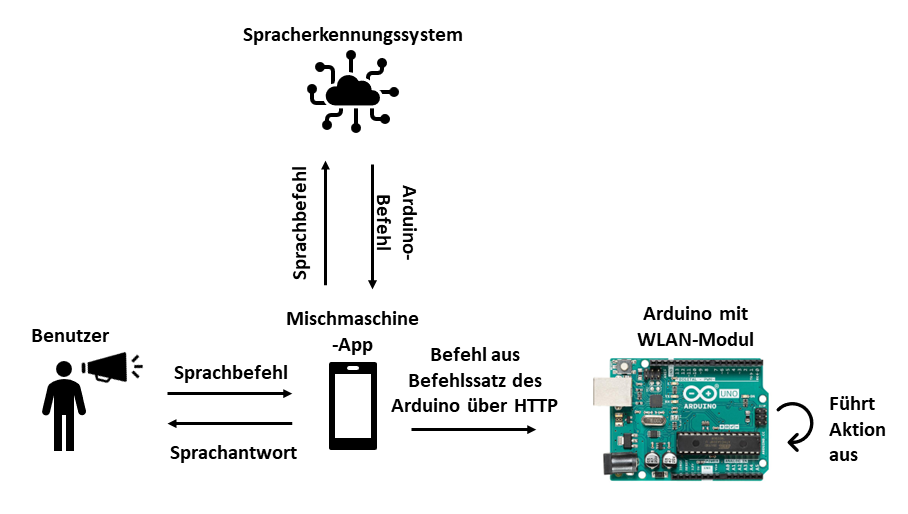
\includegraphics[width=0.8\textwidth]{Bilder_Konzept/Konzept_B.png}}
    \caption{\label{figure:Konzept_mobile_App}Spracherkennung und -verarbeitung mittels mobiler Anwendung}
\end{figure}
\noindent
Ein Problem dieser Lösung ist der offensichtliche Mehraufwand durch die Entwicklung einer eigenen Anwendung für Mobiltelefone.
Auch der Anwender hat zusätzlichen Aufwand durch die Installation.
Außerdem ist die Spracheingabe und -ausgabe über das Mobiltelefon nicht intuitiv, da der Anwender eigentlich mit der Maschine kommunizieren sollte.
Dieser Effekt kann dadurch abgeschwächt werden, dass wenigstens die Antwort durch einen Lautsprecher in der Mischmaschine an den Benutzer zurückgegeben wird.
\section{Konzept C: Spracherkennung und -verarbeitung auf Computer-Hardware}
Ein weiteres Konzept stützt sich auf die Verwendung eines Computers in der Mischmaschine anstelle eines Mikrocontrollers wie dem Arduino.
Motivation ist hierbei der Leistungsgewinn gegenüber eines Mikrocontrollers, um die Spracherkennung und -verarbeitung mittels Sprachmodell zu gewährleisten.
Ein Beispiel für einen solchen Miniaturcomputer ist der Raspberry-Pi.
Dieser bietet genügend Schnittstellen, wie etwa USB-Hubs, zum verbinden von Mikrofon als auch Lautsprecher.
Nimmt der Computer das Audiosignal auf verarbeitet er dieses und generiert daraus die Antwort, die durch den Lautsprecher ausgegeben wird, zusammen mit der Aktion für die Getränkemischmaschine.
Diese muss an den Arduino, welcher die Mischmaschine steuert, übermittelt werden.
Um dies zu ermöglichen können der Computer und der Arduino über eine serielle Schnittstelle, wie etwa einem USB-Kabel, miteinander  verbunden werden.
Abbildung \ref{figure:Konzept_Raspberry} stellt den konzeptionellen Aufbau graphisch dar.
\begin{figure}[H]
    \centering
    \fbox{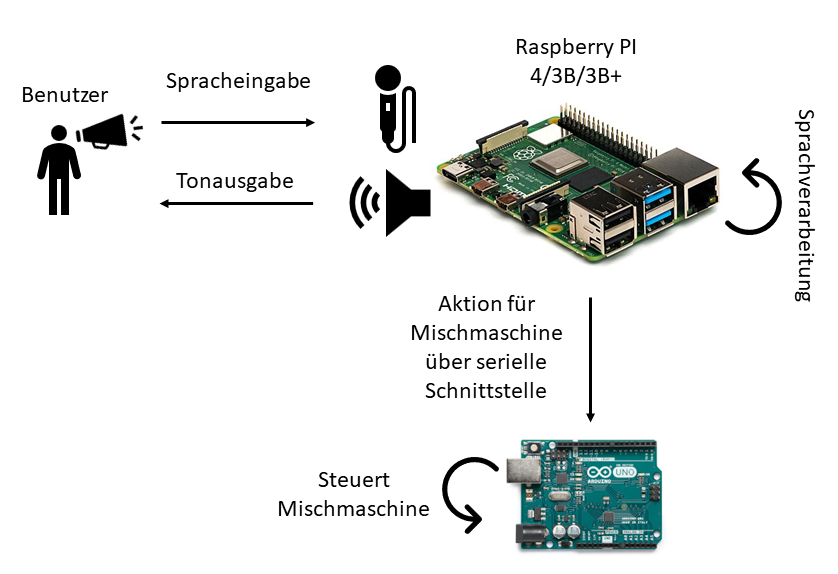
\includegraphics[width=0.8\textwidth]{Bilder_Konzept/Konzept_C.png}}
    \caption{\label{figure:Konzept_Raspberry}Spracherkennung und -verarbeitung auf Computer-Hardware}
\end{figure}
\noindent
Obwohl ein Computer wie der Raspberry-Pi im Allgemeinen eine höhere Leistung als ein Mikrocontroller hat ist damit nicht sichergestellt, dass diese zur Ausführung des Sprachmodells ausreicht.
Beispielsweise ist das vierte Modell der Raspberry-Pi-Serie mit nur maximal acht Gigabyte Arbeitsspeicher erhältlich.
Das Sprachmodell könnte allerdings noch weitaus mehr Daten im Arbeitsspeicher benötigen.
Des Weiteren ist zu beachten, dass die Miniaturcomputer von Raspberry-Pi im Speziellen zum Zeitpunkt dieser Arbeit kaum zu vertretbaren Preisen verfügbar sind.
\section{Finales Hardware-Konzept}
Die folgende Tabelle zeigt eine Übersicht bezüglich der Bewertung der einzelnen Konzepte.
\begin{table}[H]
    \centering
    \begin{tabular}{l|c|c|c|c}
        Bewertungsmatrix          & \makecell{Konzept A                                     \\ (nur Arduino)} & Konzept A & Konzept B & Konzept C \\
        \hline
        \makecell[l]{Freiheitsgrade in der Spracheingabe                                    \\ des Benutzers} & niedrig                    & sehr hoch & sehr hoch & hoch      \\
        \hline
        Hardwarekosten            & niedrig             & hoch      & niedrig   & sehr hoch \\
        \hline
        Verfügbare Rechenleistung & niedrig             & sehr hoch & sehr hoch & hoch      \\
        \hline
        Performanz                & sehr hoch           & mittel    & mittel    & sehr hoch \\
        \hline
        Overhead                  & niedrig             & hoch      & sehr hoch & niedrig   \\
    \end{tabular}
    \caption{\label{table:Bewertungsmatrix_Konzepte}Bewertung der Konzepte}
\end{table}
\noindent
Ein erster Ansatz wurde im Kapitel \ref{section:Konzept_A} zu Konzept A erläutert.
Hierbei war die Idee, die Spracherkennung und -verarbeitung nur auf dem Arduino auszuführen.
Aufgrund der mangelnden Leistung eines Arduinos können mit Hilfe von Sprachmodulen jedoch nur vordefinierte Sätze oder Wörter erkannt werden.
Damit ist der Freiheitsgrad in der Spracheingabe des Benutzers äußerst eingeschränkt.
Dafür sind die aufzuwendenden Hardwarekosten minimal.
Lediglich das Sprachmodul sowie ein Lautsprecher müssten besorgt werden.
Die Performanz wird als sehr hoch eingeschätzt, da die Spracherkennung direkt auf dem Ardunino erfolgen kann, der auch die Mischmaschine steuert.
Niedrig ist hingegen der benötigte Mehraufwand, da kaum zusätzliche Awendungen, Services oder Hardwarekomponenten benötigt werden.\\\\
Das Konzept wurde schließlich durch einen Sprachverarbeitungsservice in der Cloud ergänzt (Konzept A).
Der Benutzer hat bei diesem Ansatz große Freiheiten in seinen Formulierungen, da es kein Problem darstellt ein großes Sprachmodell in der Cloud auszuführen.
Die Hardwarekosten könnten allerdings hoch sein, je nach dem, ob der Server selbst bereitgestellt oder von einem externen Anbieter bezogen wird.
Auch die letzten Endes tatsächlich benötigte Rechenleistung spielt dabei eine Rolle.
Die verfügbare Rechenleistung ist theoretisch unbegrenzt, wobei die Performanz des Gesamtsystems nur als mittelmäßig eingestuft werden kann.
Nach der Aufnahme und eventuell einer Vorverarbeitung des Aduiosignals durch den Arduino müssen \ac{HTTP}-Nachrichten gesendet und Empfangen werden.
Je nach Last auf dem Netzwerk kann es dadurch zu Latenzen oder sogar Verbindungsabbrüchen kommen.
Außerdem ist der Overhead durch den Einsatz einer Cloud recht hoch.\\\\
Konzept B unterscheidet sich in Sachen Freiheitsgrad, Rechenleistung und Performanz nicht von Konzept A, da auch hier eine Cloud zum Einsatz kommt.
Die Hardwarekosten sind jedoch niedriger, da immerhin kein Sprachmodul, Mikrofon und Lautsprecher benötigt werden.
Die Aufgaben dieser Komponenten kann das Mobiltelefon des Anwenders übernehmen.
Der Overhead ist deutlich größer, da das Konzept die Entwicklung einer eigenen Mobilanwendung voraussetzt.\\\\
Der Freiheitsgrad wird bei Konzept C als hoch, jedoch nicht als sehr hoch, bewertet.
Grund hierfür ist die, im Vergleich zur Cloud, etwas beschränkte Leistung, welche die Leistung/Größe des Sprachmodells beeinträchtigen könnte.
Hardwarekosten können jedoch sehr hoch werden.
Bei dem Einsatz einer Cloud kann ein günstiger Anbieter gefunden werden, sodass die Anschaffung eigener Hardware entfällt.
Dies ist hier nicht der Fall.
Die Performanz des Gesamtsystems kann, wie bei Konzept A (nur mittels Arduino), sehr hoch eingeschätzt werden, da Spracherkennung und -verarbeitung direkt in der Mischmaschine von der Hardware übernommen wird.
Der Mehraufwand ist gering, da weder ein Cloudservice noch eine externe Anwendung entwickelt werden müssen.\\\\
Letzten Endes wurde das Konzept C als finales Hardware-Konzept gewählt. Wie ein Blick in die Bewertungsmatrix zeigt lässt sich dies mit den sehr guten Werten, die sich aus der Betrachtung der beschriebenen Bewertungskriterien ergaben, begründen.
\section{Konzept für die Sprachsteuerung}
\subsection{Ansatz für das Dialogsystem}
Aus dem Vergleich der wichtigsten Ansätze zur Erstellung von Chatbots, die in Kapitel \ref{sec:ansaetze_erstellung_chatbots} besprochen wurden, lassen sich die folgenden Vor- und Nachteile der einzelnen Methoden ableiten:
\begin{table}[H]
    \centering
    \begin{tabular}{m{3cm}|m{6cm}|m{6cm}}
        Ansatz               & Vorteile                                                  & Nachteile \\
        \hline
        Musterabgleich       & \makecell[l]{\tabitem Einfacher Einstieg                              \\ \tabitem Leicht wiederverwendbar\\ \tabitem Modularität\\ \tabitem Leicht zu kontrollieren/\\einzuschränken} & \makecell[l]{\tabitem Themenbereich begrenzt\\ \tabitem Die Möglichkeiten sind durch\\ die Arbeitsbelastung des\\ Entwicklers begrenzt\\ \tabitem Komplexität der Fehlersuche\\ \tabitem Strenge und \glqq{}spröde\grqq{} Regeln} \\
        \hline
        Grounding            & \makecell[l]{\tabitem Gut im Beantworten logischer\\ Fragen             \\\tabitem Leicht zu kontrollieren/\\einzuschränken}             & \makecell[l]{\tabitem Künstlicher, mechanischer Ton \\ \tabitem Probleme mit Zweideutigkeiten \\ \tabitem Probleme mit dem Allgemein-\\wissen \\ \tabitem Begrenzt auf strukturierte\\ Daten \\ \tabitem Erfordert die Extraktion von\\ Informationen in großem Umfang \\ \tabitem Erfordert menschliche Aufsicht}    \\
        \hline
        Suche                & \makecell[l]{\tabitem Einfachheit                                     \\ \tabitem Leicht zu lehren \\ \tabitem Simulation von menschlicher\\ Konversation}             & \makecell[l]{\tabitem Unzureichende Skalierung \\ \tabitem Die simulierte Persönlichkeit des\\ Bots ist inkonsistent \\ \tabitem Kennt den Kontext nicht \\ \tabitem Keine sachlichen Fragen} \\
        \hline
        \makecell[l]{Generierungs-\\methoden} & \makecell[l]{\tabitem Neue, kreative Dialoge                          \\ \tabitem Weniger Arbeit für den\\ Entwickler \\ \tabitem Kontextsensitiv}           & \makecell[l]{\tabitem Schwierig zu lehren \\ \tabitem Erfordert mehr Daten (Dialoge) \\ \tabitem Schwierig, in die richtige\\ Richtung zu lenken \\ \tabitem Erfordert mehr Rechenleistung} \\
    \end{tabular}
    \caption{\label{table:Bewertungsmatrix_Konzepte_Dialogsysteme}Bewertung der Ansätze für die Erstellung eines Dialogsystems}
\end{table}
\noindent
Bei der Analyse des Problems, ein Dialogsystem für eine Getränkmischmaschine zu entwickeln, kann man zu dem Schluss kommen, dass die beste Option eine Mischung aus dem Ansatz der Informationssuchemethode und dem Musterabgleich ist.\\\\
Das erste Argument, das für diesen Ansatz spricht, ist die Möglichkeit, die Sprachsteuerung in deutscher Sprache zu verwenden, was die Anwendung der Generierungsmethoden erschwert, da der Zugang zu einer geeigneten Datenbank in dieser Sprache, die den Anforderungen des Projekts, nämlich eine ausreichende Anzahl von Beleidigungen zu enthalten, nicht möglich ist.
Gleichzeitig können bei der Verwendung von Musterabgleich Antwortvorlagen und Muster für entsprechende Anfragen in deutscher Sprache im Voraus erstellt werden, was die Erstellung und das Training des Dialogsystems erleichtert.\\\\
Das zweite Argument ist, dass in diesem Projekt ein Raspberry Pi verwendet wird, was die Verwendung generativer Methoden aufgrund der begrenzten Hardware-Ressourcen einschränken kann.
Andererseits kann das Modell für die Informationssuche und den Musterabgleich auf Geräten mit geringem Stromverbrauch implementiert werden, was diesen Ansatz für dieses Projekt vorteilhaft macht.\\\\
Generierungsmethoden könnten auch für dieses Problem zu mächtig sein.
Beim Mixen von Cocktails können die Antworten einfach und formelhaft sein, wie z. B. \glqq{}Das hört sich eklig an, bist du sicher, dass du es willst?\grqq{} oder \glqq{}Ich hoffe, ich sehe dich nie wieder\grqq{}.
In diesem Fall kann der Einsatz von Generierungsmethoden wie seq2seq-Modellen überflüssig und ineffizient sein.
Für diese Aufgabe ist im Gegensatz zu komplexen natürlichsprachlichen Abfragen keine detaillierte semantische Verarbeitung erforderlich, so dass der Musterabgleich einen einfacheren und effizienteren Ansatz darstellt.\\\\
Bei der Verwendung des Musterabgleiches kann man den Ton und den Humor des Geräts leicht steuern und so die gewünschte Atmosphäre erzeugen.
Die Antworten des seq2seq-Modells sind wiederum sehr schwer zu steuern.
Generierungsmethoden können zu unerwünschtem Maschinenverhalten führen, wenn das Modell auf ungeeigneten Daten trainiert wird oder Fehler in der Betriebslogik enthält.
Die Verwendung einer Datenbank, die genügend Beleidigungen enthält (z. B. die 4chan-Datenbank), kann dazu führen, dass die Antworten der Maschine über das Ziel hinausschießen und statt lustig zu sein, den Benutzer beleidigen.\\\\
Mit diesem Ansatz wird auch die Effizienz der Maschinensteuerung verbessert.
Beim Musterabgleich kann eine Kategorie \glqq{}Getränkebestellung\grqq{} zugewiesen werden, die, wenn sie erkannt wird, die Maschine automatisch zur Bearbeitung der Befehle veranlasst.
Im Falle von seq2seq-Modell ist keine Kategorie vorgesehen, so dass eine zusätzliche Prüfung jeder Eingabeanweisung eingeführt werden müsste, um festzustellen, wann der Benutzer die Bestellung aufgegeben hat.\\\\
Ein letztes Argument, das für den Ansatz spricht, ist die Möglichkeit, die Maschine bei Bedarf schnell an neue Anfragen und Anforderungen anzupassen, indem neue Muster und Regeln in das System eingeführt werden.
Daher ist eine Mischung aus Informationssuchemethode und Musterabgleich für das vorliegende Problem am besten geeignet.
\subsection{Befehle}
\endinput




\chapter{Implementierung}
\section{Implementierung des Sprachverarbeitungssystems}\label{section:Implementierung_Sprachverarbeitung}
\subsection{Word2Vec-Modell}
\subsection{Sequence-to-Sequence-Modell}
\section{Implementierung der Sprachsteuerung}
Im Folgenden wird erläutert, wie die Sprachsteuerung für die Getränkemischmaschine implementiert wurde und welche Technologien dafür zum Einsatz kamen. Dabei wird zunächst auf die Spracherkennung d.h., die Umwandlung der Audiosignale (Sprachbefehl des Benutzers) in eine Form, die innerhalb des Quelltextes weiterverarbeitet werden kann, eingegangen (s. Abschnitt \ref{section:Spracherkennung}). Danach wird die Anbindung des Sprachverarbeitungssystems beschrieben, dessen Implementierung in Abschnitt \ref{section:Implementierung_Sprachverarbeitung} erklärt wird. Abschließend wird die Kommunikation mit der Mischmaschine über den Arduino illustriert (s. Abschnitt \ref{section:Befehlsverarbeitung}).
\subsection{Spracherkennung}\label{section:Spracherkennung}
Die Spracherkennung ist der erste Schritt bei der Implementierung einer Sprachsteuerung für die Getränkemischmaschine. Mit Spracherkennung ist die Aufnahme eines Tonsignals über ein Audio-Eingabegerät (Mikrofon) und die Umwandlung der Audiodaten in Text gemeint. Der Quelltext zur Implementierung der Sprachsteuerung erfolgt mit der Programmiersprache \textit{Python}, da hier sehr viele, leicht zu bedienende Bibliotheken zur Spracherkennung, -verarbeitung und \ac{KI} zur Verfügung stehen.\\\\
Für dieses Projekt viel die Wahl auf das Paket \textit{SpeechRecognition}, das die Verwendung verschiedener Spracherkennungsdienste über eine einheitliche Schnittstelle ermöglicht und zu diesem Zweck auch zur Aufnahme und Verarbeitung der Audiosignale verwendet werden kann \cite{speechrecognition}. Ein großer Vorteil davon ist, dass dadurch ein schneller Wechsel der eingesetzten \ac{API} erfolgen kann, sollte dies erforderlich sein. Die Verwendung des \textit{SpeechRecognition}-Pakets findet fast ausschließlich über die \textit{Recognizer}-Klasse statt. Um Audiosignale über eine physische Audioquelle (bspw. ein Mikrofon am Computer) aufzunehmen kann die \textit{Microphone}-Klasse verwendet werden, die ebenfalls im Paket enthalten ist. Mit Hilfe eines Objekts vom Typ \textit{Microphone} und der Methode \textit{listen} der \textit{Recognizer}-Klasse können anschließend Audiodaten aufgenommen werden, die in einem Objekt vom Typ \textit{AudioData} gespeichert sind. Die Verwendung von \textit{Recognizer} und \textit{Microphone} sind in Listing \ref{speech_rec_1} zu sehen. 
\lstinputlisting[language=python, style=algoBericht, label={speech_rec_1}, basicstyle=\tiny\sffamily, captionpos=b, caption={Audioaufnahme mit \textit{SpeechRecognition}}]{./Listings/speech_rec_1.py}
Das \textit{AudioData}-Objekt kann nun verwendet werden um die darin gespeicherten Audiodaten zu erkennen und in Text umzuwandeln. Das \textit{SpeechRecognition}-Paket stellt dafür verschiedene Möglichkeiten zur Verfügung, wie eingangs erwähnt wurde. Diese sollen im Folgenden kurz beschrieben werden:
\begin{itemize}
    \item Whisper: Whisper ist ein neuronales Netz das von der Firma \textit{OpenAI} trainiert und als Open-Source-Projekt zur Verfügung gestellt wird \cite{openai,whisper}. Neben der Fähigkeit Sprache in Text zu konvertieren kann es auch eingesetzt werden um Transkripte zu generieren, die gesprochene Sprache automatisch zu erkennen oder in die englische Sprache zu übersetzen. Das Paket \textit{SpeechRecognition} lässt sowohl die Verwendung der von \textit{OpenAI} zur Verfügung gestellten Online-\ac{API} zu, als auch die lokale Ausführung des Sprachmodells. Aufgrund der Anforderung nach Offline-Funktionalität entfällt die erste Möglichkeit (s. Kapitel \ref{chap:Anforderungen}).
    \item Google: \textit{SpeechRecognition} bietet zwei Möglichkeiten Google-Dienste zur Konvertierung von Sprache zu Text zu verwenden. Die erste Möglichkeit besteht in der Verwendung der \textit{Google Speech API} in der \textit{Google Cloud} \cite{google_cloud_speech}. Die zweite Möglichkeit besteht in der Verwendung der \textit{Google Speech API} ohne die \textit{Google Cloud}. Die Verwendung der Google-Schnittstelle entfällt jedoch für dieses Projekt, da eine aktive Internetverbindung Voraussetzung dafür ist. Außerdem sind die Google-Dienste weder kostenfrei noch open-source.
    \item Sphinx:
    \item Microsoft:
\end{itemize}
Die einzelnen \ac{API}s lassen sich jeweils über einen Methodenaufruf der Form \textit{Recognizer.recognize\_x} verwenden, wobei das \glqq{}x\grqq{} für den Namen der jeweiligen \ac{API} steht. Für dieses Projekt viel die Wahl auf die Verwendung der \textit{Whisper}-Bibliothek von \textit{OpenAI}. Dies ist damit zu begründen, dass...
\lstinputlisting[language=python, style=algoBericht, label={speech_rec_2}, basicstyle=\tiny\sffamily, captionpos=b, caption={Sprache zu Text mit \textit{OpenAI Whisper}}]{./Listings/speech_rec_2.py}
\subsubsection{Herausforderungen bei der Implementierung der Spracherkennung}
Installation von Whisper bzw. PyTorch
\subsection{Anbindung des Sprachmodells an die Mischmaschine}
\subsection{Befehlsverarbeitung in der Mischmaschine}\label{section:Befehlsverarbeitung}
\endinput



\chapter{Fazit und Ausblick}

TODO





% Ab hier beginnt der Anhang
\pagenumbering{roman}
\setcounter{page}{\value{roman-numbering}}
\appendix
% \addcontentsline{toc}{chapter}{Anhang}

% \addcontentsline{toc}{chapter}{Index}
\printindex

\addcontentsline{toc}{chapter}{Literaturverzeichnis}

% Haben Sie das "biblatex"-Paket nicht installiert, benutzen Sie folgendes:
% Ohne das "biblatex"-Paket (s. bericht.sty) produziert folgendes
% "deutsche" Zitate in Literaturverzeichnissen gemaß der Norm DIN 1505,
% Teil 2 vom Jan. 1984.
% Die Zitatmarken werden alphabetisch nach Verfassern
% sortiert und sind durch abgekürzte Verfasserbuchstaben plus
% Erscheinungsjahr in eckigen Klammern gekennzeichnet.

% \bibliographystyle{alphadin}
% \bibliography{bericht}

%%%%%%%%%%%%%%%%%%%%%%%%%%%%%%%%%%%%%%%5
% BIBLATEX
% Benutzt man das "biblatex"-Paket, muß man folgendes schreiben:
\def\refname{Literaturverzeichnis}
\printbibliography
%%%%%%%%%%%%%%%%%%%%%%%%%%%%%%%%%%%%%%%5


%%%%%%%%%%%%%%%%%%%%%%%%%%%%%%%%%%%%%%%%%%%%%%%%%%%%%%%%%%%%%%%%%%%%%%%%%%%%%%%%
%% Descr:       Vorlage für Berichte der DHBW-Karlsruhe, Änderungshistorie
%% Author:      Prof. Dr. Jürgen Vollmer, vollmer@dhbw-karlsruhe.de
%% $Id: changelog.tex,v 1.16 2020/03/13 15:12:39 vollmer Exp $
%% -*- coding: utf-8 -*-
%%%%%%%%%%%%%%%%%%%%%%%%%%%%%%%%%%%%%%%%%%%%%%%%%%%%%%%%%%%%%%%%%%%%%%%%%%%%%%%

\chapter*{Änderungen}

\begin{description}
\item[2020/03/13] Tippfehler korrigiert\\
                  aktuelle Formulierungen aus der Prüfungsordnung Technik übernommen\\
                  Formatdatei erklärt
\item[2017/10/06] Anpassung an neuer Versionen diverse Pakete.
\item[2016/03/16] Auf UTF-8 umgestellt, Indices.
\item[2010/04/12] ToDo-Markierungen mit dem \verb+\todo+-Kommando.
\item[2010/01/27] Anhang (\texttt{appendix}), Selbständigkeits-Erklärung, \texttt{framed}-Paket.
\item[2010/01/21] Abkürzungen (\texttt{acronym}), \texttt{table} und \texttt{tabular} benutzt,
     unübliche Pakete beigelegt.
\item[2010/01/18] Code-Listings (\texttt{listings}), Literaturreferenzen \texttt{biblatex})
\item[2010/01/11] Initiale Version.
\end{description}


\newpage
\addcontentsline{toc}{chapter}{Liste der ToDo's}
\listoftodos[Liste der ToDo's]


\end{document}
